\documentclass[a4paper]{article}

% CJK support: prefer ctex, fallback to XeTeX native line breaking
\IfFileExists{ctex.sty}{
  \usepackage[fontset=fandol]{ctex}
}{
  % Fallback for minimal TeX installs (e.g. MacTeX Basic, TeX Live scheme-basic)
  % without ctex/xeCJK. Uses XeTeX's built-in CJK line breaking.
  \usepackage{fontspec}
  \XeTeXlinebreaklocale "zh"
  \XeTeXlinebreakskip = 0pt plus 1pt
  \IfFontExistsTF{Songti SC}{\setmainfont{Songti SC}}{%
    \IfFontExistsTF{Noto Serif CJK SC}{\setmainfont{Noto Serif CJK SC}}{}%
  }
  \IfFontExistsTF{Heiti SC}{\setsansfont{Heiti SC}}{%
    \IfFontExistsTF{Noto Sans CJK SC}{\setsansfont{Noto Sans CJK SC}}{}%
  }
}

% Basic packages
\usepackage{amsmath, amssymb}
\usepackage{graphicx}
\usepackage[margin=2.5cm]{geometry}
\emergencystretch=3em
\usepackage[most]{tcolorbox}
\usepackage{etoolbox}
\usepackage{listings}
\usepackage{hyperref}
\usepackage{booktabs}
\usepackage{array}
\usepackage{subcaption}
\usepackage{float}
\usepackage{tikz}
\IfFileExists{pgfplots.sty}{
    \usepackage{pgfplots}
    \pgfplotsset{compat=1.18}
}{}

% ===== Highlight boxes =====
\newtcolorbox{knowledgebox}[1]{
    enhanced, colback=blue!5!white, colframe=blue!75!black, colbacktitle=blue!75!black,
    coltitle=white, fonttitle=\bfseries, title={#1}, attach boxed title to top left={yshift=-2mm, xshift=2mm},
    boxrule=1pt, sharp corners
}

\newtcolorbox{importantbox}[1]{
    enhanced, colback=yellow!10!white, colframe=yellow!80!black, colbacktitle=yellow!80!black,
    coltitle=black, fonttitle=\bfseries, title={#1}, sharp corners
}

\newtcolorbox{warningbox}[1]{
    enhanced, colback=red!5!white, colframe=red!75!black, colbacktitle=red!75!black,
    coltitle=white, fonttitle=\bfseries, title={#1}, sharp corners
}

\newtcolorbox{practicebox}[1]{
    enhanced, colback=black!3!white, colframe=black!75, colbacktitle=black!75,
    coltitle=white, fonttitle=\bfseries, title={#1}, sharp corners
}

% ===== Code listings =====
\lstset{
    basicstyle=\ttfamily\small,
    keywordstyle=\color{blue},
    stringstyle=\color{red!60!black},
    commentstyle=\color{green!60!black},
    breaklines=true,
    frame=single,
    numbers=left,
    numberstyle=\tiny\color{gray},
    captionpos=b,
    extendedchars=false
}

% ===== Figure provenance and unit macros =====
% \vtag goes inside \caption{...}; \srcnote{MM:SS--MM:SS} follows the figure environment.
\newcommand{\vtag}{\protect\footnotemark}
\newcommand{\srcnote}[1]{\footnotetext{视频画面时间区间：#1。若为裁剪图，时间区间仍对应原视频画面。}}
% Units work in text and math mode; never hand-write $^\circ$ or \AA inside \mathrm.
\newcommand{\degC}{\ensuremath{^{\circ}\mathrm{C}}}
\newcommand{\um}{\ensuremath{\mu\mathrm{m}}}
\newcommand{\nm}{\ensuremath{\mathrm{nm}}}
\newcommand{\angstrom}{\ensuremath{\text{\AA}}}

% ===== Front-page metadata =====
% Fill these in when generating notes.
\newcommand{\notetitle}{线性代数基础（二）}
\newcommand{\notesubtitle}{GAMES001 图形学中的数学 · 第 2 集：矩阵分解、范数、矩阵求导与张量}
\newcommand{\noteauthors}{根据 GAMES-Webinar 直播录像整理（倪星宇 主讲）}
\newcommand{\notedate}{2024年3月11日（直播）}
\newcommand{\videochannel}{GAMES-Webinar（哔哩哔哩）}
\newcommand{\videopublishdate}{2024年3月6日（合集）}
\newcommand{\videoduration}{2小时15分19秒}
\newcommand{\videourl}{https://www.bilibili.com/video/BV1MF4m1V7e3/?p=2}
\newcommand{\videocoverpath}{cover.jpg}

\begin{document}

% ===== Title page =====
\begin{titlepage}
\centering
{\Large 课程笔记\par}
\vspace{1.2cm}
{\huge\bfseries \notetitle\par}
\ifdefempty{\notesubtitle}{}{
\vspace{0.3cm}
{\large \notesubtitle\par}
}
\vspace{0.5cm}
{\large \noteauthors\par}
\vspace{0.3cm}
{\large \notedate\par}
\vspace{1.0cm}

\ifdefempty{\videocoverpath}{
{\small 请在生成笔记时填入视频封面图的本地路径。\par}
}{
\includegraphics[width=0.82\textwidth,height=0.40\textheight,keepaspectratio]{\videocoverpath}\par
}

\vfill
\begin{tcolorbox}[width=0.9\textwidth, colback=black!2!white, colframe=black!60, sharp corners]
\textbf{视频作者/频道}：\videochannel\par
\textbf{发布日期}：\videopublishdate\par
\textbf{视频时长}：\videoduration\par
\textbf{视频链接}：
\ifdefempty{\videourl}{
未填写
}{
\href{\videourl}{\nolinkurl{\videourl}}
}
\end{tcolorbox}
\end{titlepage}

\tableofcontents
\newpage

%% --- 正文内容开始 --- %%

\section{这一讲要补齐什么}

第二讲接着上一讲没有讲完的线性代数，覆盖四块内容：矩阵分解、向量与矩阵的范数、矩阵求导，以及内积、外积、向量积与张量。倪星宇在开场对课程定位做了澄清：这门课的目的不是把每一门数学从头到尾讲完，那不现实；它更像一份“工具书”式的索引，告诉读者图形学会用到哪些数学工具、需要掌握到什么程度，以及遇到问题时去哪里查。这一讲他换了收音更好的设备，还准备了手写板，因为本讲有不少推导需要在课件上直接演算。

本讲义的读者只需要上一讲的内容作为前提：矩阵是线性映射的表示，内积给出长度与夹角，正定矩阵对应“恒正的二次型”。读完以后，读者应能：用 LU、Cholesky、QR、SVD 四种分解说明“为什么要分解矩阵”；区分向量范数、诱导范数、元素形式范数与 Schatten 范数；用“微分—迹”的技巧推导常见的矩阵导数，并据此推出最小二乘的正规方程；理解协变与逆变、并矢、缩并与 Levi-Civita 符号，并用张量记号证明向量恒等式。

\subsection{关于 GAMES002 与跨平台工具}

开课前，倪星宇回答了弹幕中关于 GAMES002（图形学工具课）的提问。他参与过 GAMES002 的提出与建设，原因是他们在北大开图形学课时发现，许多同学卡在开发环境上：有同学带着 Mac 来上课，问为什么某些工具装不上。因此 GAMES002 推荐的工具都尽量容易跨平台。他举了 OpenGL 的例子：只有 Windows 与原生 Linux 支持 OpenGL 的最新版本 4.6，Mac 的支持停留在 4.1；Mac 有自己的图形 API Metal，但普及率有限。

\subsection{本章小结}

这一讲的四块内容彼此衔接：矩阵分解提供高效求解与几何解释，范数提供衡量误差与收敛的尺子，矩阵求导把优化与物理模拟中的“对矩阵求导”变成可操作的规则，张量则统一了内积、叉积与更高阶的物理量。下面先从矩阵分解开始。

\section{矩阵分解：把一个矩阵拆成好算的几块}

矩阵分解（decomposition）把一个矩阵写成若干个结构简单的矩阵之积，例如三角矩阵、正交（幺正）矩阵或对角矩阵。三角矩阵的方程可以逐个代入求解，正交矩阵的逆就是转置，对角矩阵只做缩放。分解之后，原来困难的问题被拆成若干个容易的问题。

\subsection{PLU 分解与高斯消元}

PLU 分解写作
\[
\boldsymbol A=\boldsymbol P\boldsymbol L\boldsymbol U ,
\]
\begin{itemize}
\item $\boldsymbol A$：方阵；$\boldsymbol P$：初等变换（行置换）矩阵；$\boldsymbol L$：下三角矩阵；$\boldsymbol U$：上三角矩阵。
\end{itemize}
当 $\boldsymbol P$ 取单位矩阵时，退化为 LU 分解。它的应用是用高斯消元求解矩阵方程。倪星宇在手写板上用一个 $3\times3$ 的例子说明“高斯消元等价于 LU 分解”：
\[
\boldsymbol A=\begin{pmatrix}9&6&0\\6&5&4\\3&4&10\end{pmatrix}.
\]
\begin{itemize}
\item $\boldsymbol A$：待分解的矩阵，第一列主元为 9。
\end{itemize}
第一步把第一行乘以 $-2/3$ 加到第二行，对应左乘初等矩阵 $\boldsymbol E_0$；第二步把第一行乘以 $-1/3$ 加到第三行，对应 $\boldsymbol E_1$；第三步把第二行乘以 $-2$ 加到第三行，对应 $\boldsymbol E_2$：
\[
\boldsymbol E_0=\begin{pmatrix}1&0&0\\-\tfrac23&1&0\\0&0&1\end{pmatrix},\quad
\boldsymbol E_1=\begin{pmatrix}1&0&0\\0&1&0\\-\tfrac13&0&1\end{pmatrix},\quad
\boldsymbol E_2=\begin{pmatrix}1&0&0\\0&1&0\\0&-2&1\end{pmatrix}.
\]
\begin{itemize}
\item $\boldsymbol E_0,\boldsymbol E_1,\boldsymbol E_2$：依次消去 $(2,1)$、$(3,1)$、$(3,2)$ 位置元素的初等变换矩阵，都是下三角矩阵。
\end{itemize}
中间结果依次为 $\boldsymbol A_0=\boldsymbol E_0\boldsymbol A$、$\boldsymbol A_1=\boldsymbol E_1\boldsymbol A_0$、$\boldsymbol A_2=\boldsymbol E_2\boldsymbol A_1$，最终
\[
\boldsymbol U=\boldsymbol A_2=\boldsymbol E_2\boldsymbol E_1\boldsymbol E_0\boldsymbol A=\begin{pmatrix}9&6&0\\0&1&4\\0&0&2\end{pmatrix},
\qquad
\boldsymbol A=(\boldsymbol E_2\boldsymbol E_1\boldsymbol E_0)^{-1}\boldsymbol U=\boldsymbol L\boldsymbol U .
\]
\begin{itemize}
\item $\boldsymbol U$：消元得到的上三角矩阵；$\boldsymbol L=(\boldsymbol E_2\boldsymbol E_1\boldsymbol E_0)^{-1}$：下三角矩阵的积的逆，仍是下三角矩阵。
\end{itemize}
讲者的论证是：每个 $\boldsymbol E_i$ 都是下三角矩阵，下三角矩阵之积仍是下三角，其逆也是下三角，所以每做一次高斯消元，就等价于做了一次 LU 分解。按本例可以算出 $\boldsymbol L=\begin{pmatrix}1&0&0\\ 2/3&1&0\\ 1/3&2&1\end{pmatrix}$（讲义作者验算）。$\boldsymbol P$ 的作用是什么？上面的消元只用到了“某一行乘以一个数加到另一行”，没有交换行；当某个主元为零、需要交换行时，交换操作就记录在 $\boldsymbol P$ 中，于是得到 PLU 分解。

\noindent\begin{minipage}{\textwidth}
\begin{figure}[H]
\centering
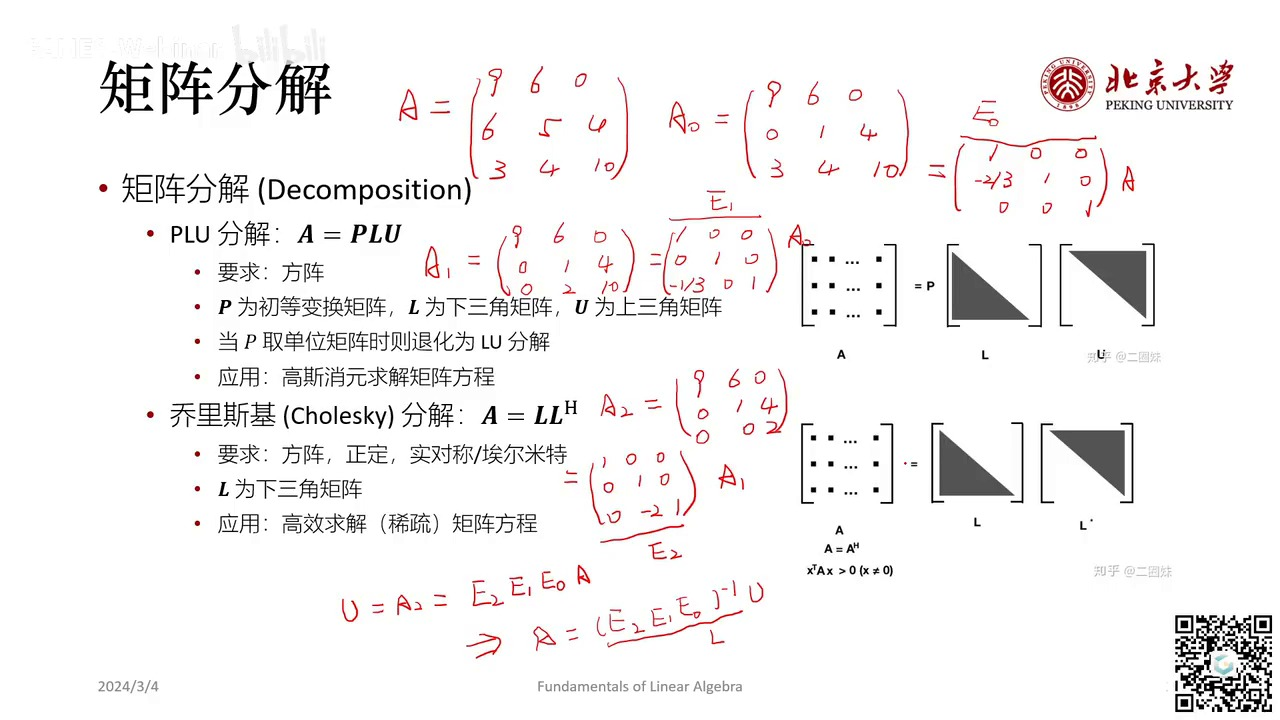
\includegraphics[width=0.92\textwidth]{figures/fig_01_lu_example.jpg}
\caption{手写板上的 LU 分解示例：三次初等行变换把 $\boldsymbol A$ 消成上三角矩阵 $\boldsymbol U$，$\boldsymbol A=(\boldsymbol E_2\boldsymbol E_1\boldsymbol E_0)^{-1}\boldsymbol U$\vtag}
\end{figure}
\srcnote{00:16:00--00:16:15}
\end{minipage}


有了 $\boldsymbol A=\boldsymbol L\boldsymbol U$，求解 $\boldsymbol A\boldsymbol x=\boldsymbol b$ 就拆成两次三角回代：
\[
\boldsymbol L(\boldsymbol U\boldsymbol x)=\boldsymbol b\ \Rightarrow\ \boldsymbol L\boldsymbol y=\boldsymbol b,\qquad \boldsymbol U\boldsymbol x=\boldsymbol y .
\]
\begin{itemize}
\item $\boldsymbol y=\boldsymbol U\boldsymbol x$：中间变量；先由下三角方程前代得 $\boldsymbol y$，再由上三角方程回代得 $\boldsymbol x$。
\end{itemize}
讲者说，用 LU 分解解方程，本质上就是用高斯消元解方程。分解的好处在于可以复用：同一个 $\boldsymbol A$ 对应多个右端 $\boldsymbol b$ 时，只需分解一次，之后每个 $\boldsymbol b$ 只做两次三角回代。

\begin{practicebox}{课上的三个手算例题}
\begin{itemize}
\item LU：用三次初等行变换把 $\begin{pmatrix}9&6&0\\6&5&4\\3&4&10\end{pmatrix}$ 消成上三角，记录每次变换的矩阵，乘积的逆即 $\boldsymbol L$。
\item Cholesky：验证 $\begin{pmatrix}4&12&-16\\12&37&-43\\-16&-43&98\end{pmatrix}$ 等于下三角矩阵与其转置之积。
\item QR：对 $\begin{pmatrix}1&2&2\\2&1&2\\1&2&1\end{pmatrix}$ 的三列做施密特正交化，再归一化得到 $\boldsymbol Q$，用投影系数与长度拼出 $\boldsymbol R$。
\end{itemize}
\end{practicebox}

\subsection{Cholesky 分解}

乔里斯基（Cholesky）分解写作 $\boldsymbol A=\boldsymbol L\boldsymbol L^{\mathrm H}$，要求 $\boldsymbol A$ 为方阵、正定、实对称或埃尔米特，$\boldsymbol L$ 为下三角矩阵，应用是高效求解（稀疏）矩阵方程。它在形式上与 LU 一样是“下三角乘上三角”，不同之处在于上下两个三角矩阵互为（共轭）转置。课上给出的例子是
\[
\begin{pmatrix}4&12&-16\\12&37&-43\\-16&-43&98\end{pmatrix}
=\begin{pmatrix}2&0&0\\6&1&0\\-8&5&3\end{pmatrix}
\begin{pmatrix}2&6&-8\\0&1&5\\0&0&3\end{pmatrix}.
\]
\begin{itemize}
\item 左侧：对称正定矩阵；右侧第一个因子为 $\boldsymbol L$，第二个为 $\boldsymbol L^{\mathsf T}$。
\end{itemize}
讲者解释了 Cholesky 分解为何有自己的算法：利用实对称、正定这些性质，$n$ 阶方阵的 Cholesky 分解可以归约为 $n-1$ 阶方阵的 Cholesky 分解，逐级递推求出：先由左上角元素开平方得到 $\boldsymbol L$ 的第一个对角元，再用它求出第一列，剩下的右下角子矩阵减去第一列的外积后仍对称正定，于是问题缩小一阶。课上的例子正可以这样验算：$\sqrt4=2$，$12/2=6$，$-16/2=-8$，以此类推。求解方程时与 LU 相同，只需把 $\boldsymbol U$ 换成 $\boldsymbol L^{\mathsf T}$。

\noindent\begin{minipage}{\textwidth}
\begin{figure}[H]
\centering
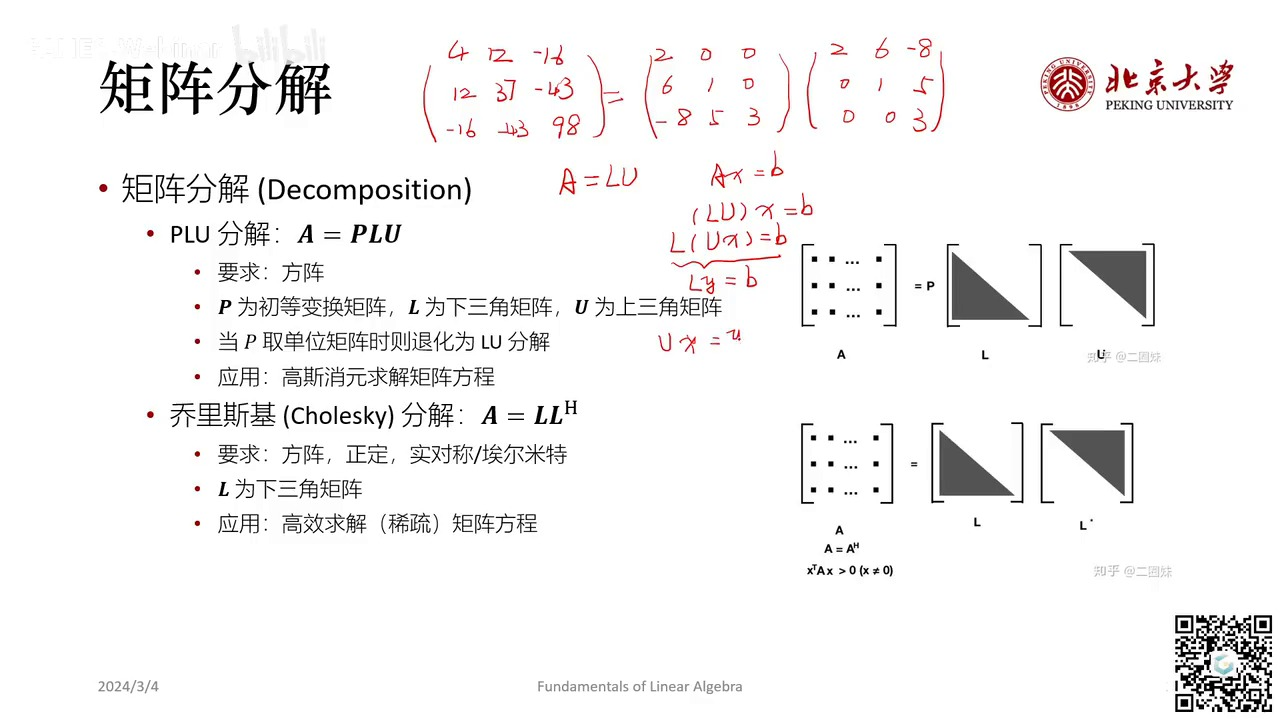
\includegraphics[width=0.92\textwidth]{figures/fig_02_cholesky_example.jpg}
\caption{Cholesky 分解示例，以及用 $\boldsymbol A=\boldsymbol L\boldsymbol U$ 把 $\boldsymbol A\boldsymbol x=\boldsymbol b$ 拆成 $\boldsymbol L\boldsymbol y=\boldsymbol b$ 与 $\boldsymbol U\boldsymbol x=\boldsymbol y$\vtag}
\end{figure}
\srcnote{00:22:00--00:22:15}
\end{minipage}


\begin{warningbox}{关于复杂度的说法}
讲者在课上提到 Cholesky 分解利用对称性归约子问题，“复杂度一般来说是 $n^2$ 的，降了一级”。讲义作者补充：对稠密矩阵，Cholesky 分解的计算量通常仍是 $O(n^3)$ 量级，约为 LU 分解的一半；它的优势在于只需存一半元素、数值稳定且无需选主元，对稀疏矩阵还能配合重排序保持稀疏性。三角回代本身才是 $O(n^2)$。
\end{warningbox}

\subsection{QR 分解}

QR 分解写作 $\boldsymbol A=\boldsymbol Q\boldsymbol R$，要求 $\boldsymbol A_{m\times n}$ 列满秩且 $m\ge n$；$\boldsymbol Q_{m\times m}$ 为幺正矩阵，$\boldsymbol R_{m\times n}$ 为上三角矩阵；非方阵时 $\boldsymbol R$ 的下半部分为零矩阵。求解方法有施密特正交化、吉文斯（Givens）变换或豪斯霍尔德（Householder）变换；应用包括高效求解（稠密）矩阵方程，以及分解形变梯度。

后一个应用来自物理模拟：软体的形变梯度中含有旋转部分，把旋转部分提出来，剩下的才是真正的变形。讲者解释，如果形变全是旋转，那对应的是刚体运动，不产生弹性力；因此要把旋转与真正的伸缩分开处理。

课上用施密特正交化演示了 QR 分解。取
\[
\boldsymbol A=\begin{pmatrix}1&2&2\\2&1&2\\1&2&1\end{pmatrix},\qquad
\begin{aligned}
\boldsymbol b_1&=\boldsymbol a_1=(1,2,1),\\
\boldsymbol b_2&=\boldsymbol a_2-\boldsymbol b_1=(1,-1,1),\\
\boldsymbol b_3&=\boldsymbol a_3-\tfrac13\boldsymbol b_2-\tfrac76\boldsymbol b_1=\left(\tfrac12,0,-\tfrac12\right),
\end{aligned}
\]
\begin{itemize}
\item $\boldsymbol a_i$：$\boldsymbol A$ 的第 $i$ 列；$\boldsymbol b_i$：正交化后的向量；系数 $1$、$\tfrac13$、$\tfrac76$ 分别是 $\boldsymbol a_2$ 在 $\boldsymbol b_1$ 上、$\boldsymbol a_3$ 在 $\boldsymbol b_2$ 和 $\boldsymbol b_1$ 上的投影系数。
\end{itemize}
再把 $\boldsymbol b_i$ 归一化，得到
\[
\boldsymbol Q=\begin{pmatrix}1/\sqrt6&1/\sqrt3&1/\sqrt2\\2/\sqrt6&-1/\sqrt3&0\\1/\sqrt6&1/\sqrt3&-1/\sqrt2\end{pmatrix},\qquad
\boldsymbol R=\begin{pmatrix}\sqrt6&\sqrt6&7/\sqrt6\\0&\sqrt3&1/\sqrt3\\0&0&1/\sqrt2\end{pmatrix}.
\]
\begin{itemize}
\item $\boldsymbol Q$ 的各列是单位正交向量；$\boldsymbol R$ 的对角元是各 $\boldsymbol b_i$ 的长度，非对角元是投影系数乘以对应长度。
\end{itemize}

\noindent\begin{minipage}{\textwidth}
\begin{figure}[H]
\centering
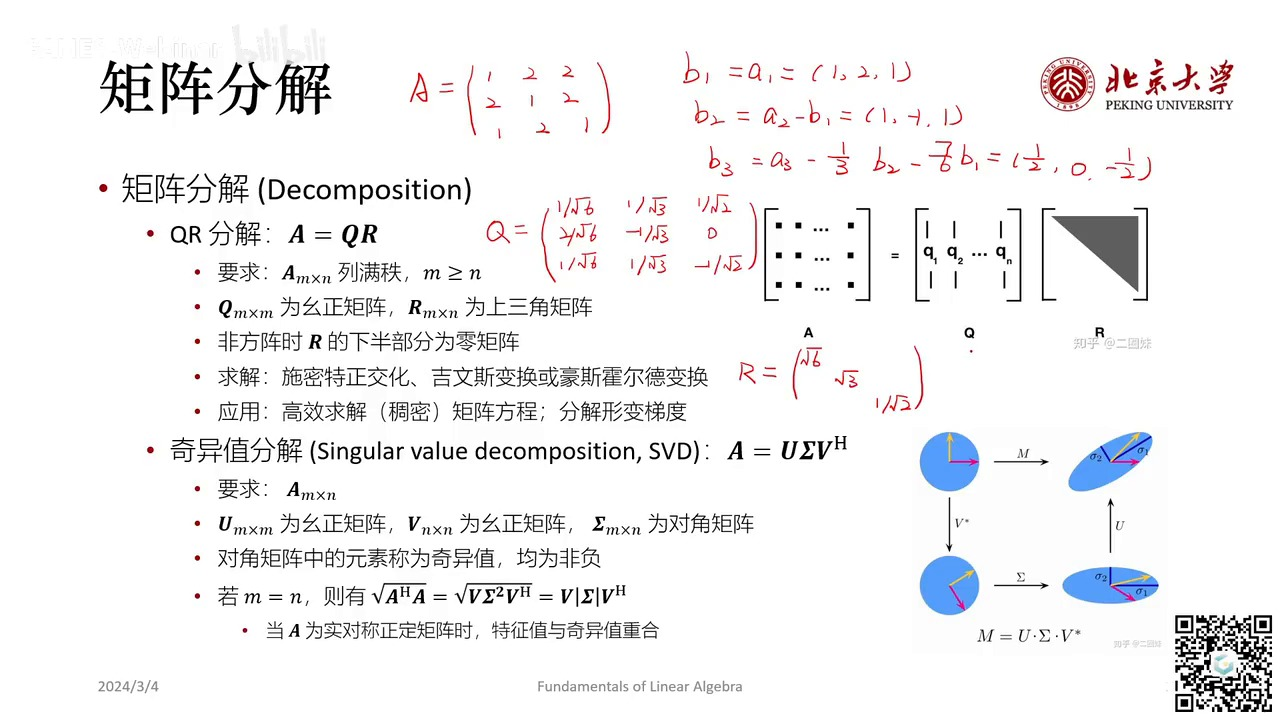
\includegraphics[width=0.92\textwidth]{figures/fig_03_qr_example.jpg}
\caption{手写板上的 QR 分解示例：先施密特正交化得到 $\boldsymbol b_1,\boldsymbol b_2,\boldsymbol b_3$，再归一化得到 $\boldsymbol Q$ 与 $\boldsymbol R$\vtag}
\end{figure}
\srcnote{00:27:00--00:27:15}
\end{minipage}


\subsection{奇异值分解}

讲者称奇异值分解（SVD）是做 CV 也好、做 CG 也好都不得不接触的一种分解：
\[
\boldsymbol A=\boldsymbol U\boldsymbol\Sigma\boldsymbol V^{\mathrm H},
\]
\begin{itemize}
\item $\boldsymbol A_{m\times n}$：任意矩阵；$\boldsymbol U_{m\times m}$、$\boldsymbol V_{n\times n}$：幺正矩阵；$\boldsymbol\Sigma_{m\times n}$：对角矩阵，其对角元称为奇异值，均为非负。
\end{itemize}
课件上的示意图从几何上解释 SVD：一个单位圆先经过 $\boldsymbol V^{*}$ 旋转，再经过 $\boldsymbol\Sigma$ 沿坐标轴缩放（在 $x$ 方向拉伸、$y$ 方向压缩），最后经过 $\boldsymbol U$ 再旋转一次，得到与直接作用 $\boldsymbol M$ 相同的椭圆。任何线性变换都可以拆成“旋转—缩放—旋转”。

\noindent\begin{minipage}{\textwidth}
\begin{figure}[H]
\centering
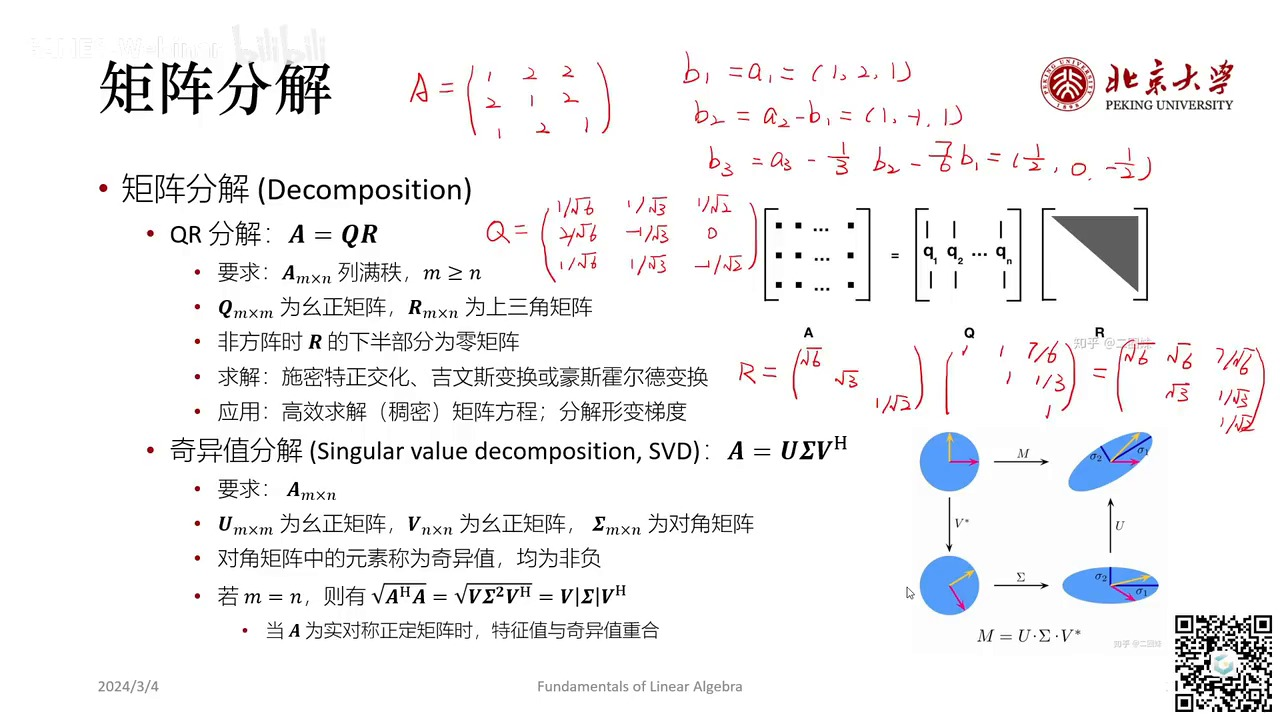
\includegraphics[width=0.92\textwidth]{figures/fig_04_svd_geometry.jpg}
\caption{QR 分解与奇异值分解：SVD 把任意线性变换拆成旋转 $\boldsymbol V^{*}$、轴向缩放 $\boldsymbol\Sigma$ 与旋转 $\boldsymbol U$\vtag}
\end{figure}
\srcnote{00:28:00--00:28:15}
\end{minipage}


奇异值与特征值有什么关系？当 $m=n$ 时，
\[
\sqrt{\boldsymbol A^{\mathrm H}\boldsymbol A}=\sqrt{\boldsymbol V\boldsymbol\Sigma^2\boldsymbol V^{\mathrm H}}=\boldsymbol V|\boldsymbol\Sigma|\boldsymbol V^{\mathrm H}.
\]
\begin{itemize}
\item $\boldsymbol A^{\mathrm H}\boldsymbol A$：半正定的埃尔米特矩阵；$|\boldsymbol\Sigma|$：奇异值组成的对角矩阵。
\end{itemize}
讲者的解读是：$\boldsymbol V$ 是旋转矩阵，$\boldsymbol V^{\mathrm H}$ 是它的逆，中间剩下的对角元就是 $\sqrt{\boldsymbol A^{\mathrm H}\boldsymbol A}$ 的特征值，因为任何能通过相似变换化为对角矩阵的矩阵，其对角元就对应特征值。所以奇异值是 $\sqrt{\boldsymbol A^{\mathrm H}\boldsymbol A}$ 的特征值。当 $\boldsymbol A$ 为实对称正定矩阵时，特征值与奇异值重合；反过来说，如果矩阵不是正定的，特征值与奇异值可能不同，这时尤其需要小心。

\begin{warningbox}{特征值与奇异值不要混用}
特征值来自相似变换 $\boldsymbol P^{-1}\boldsymbol A\boldsymbol P$，可以为负数或复数，只对方阵有定义；奇异值来自 $\boldsymbol U\boldsymbol\Sigma\boldsymbol V^{\mathrm H}$，总是非负实数，对任意 $m\times n$ 矩阵都有定义。只有实对称正定（或更一般的埃尔米特半正定）矩阵，两者才逐一重合。
\end{warningbox}

\noindent\begin{minipage}{\textwidth}
\begin{figure}[H]
\centering
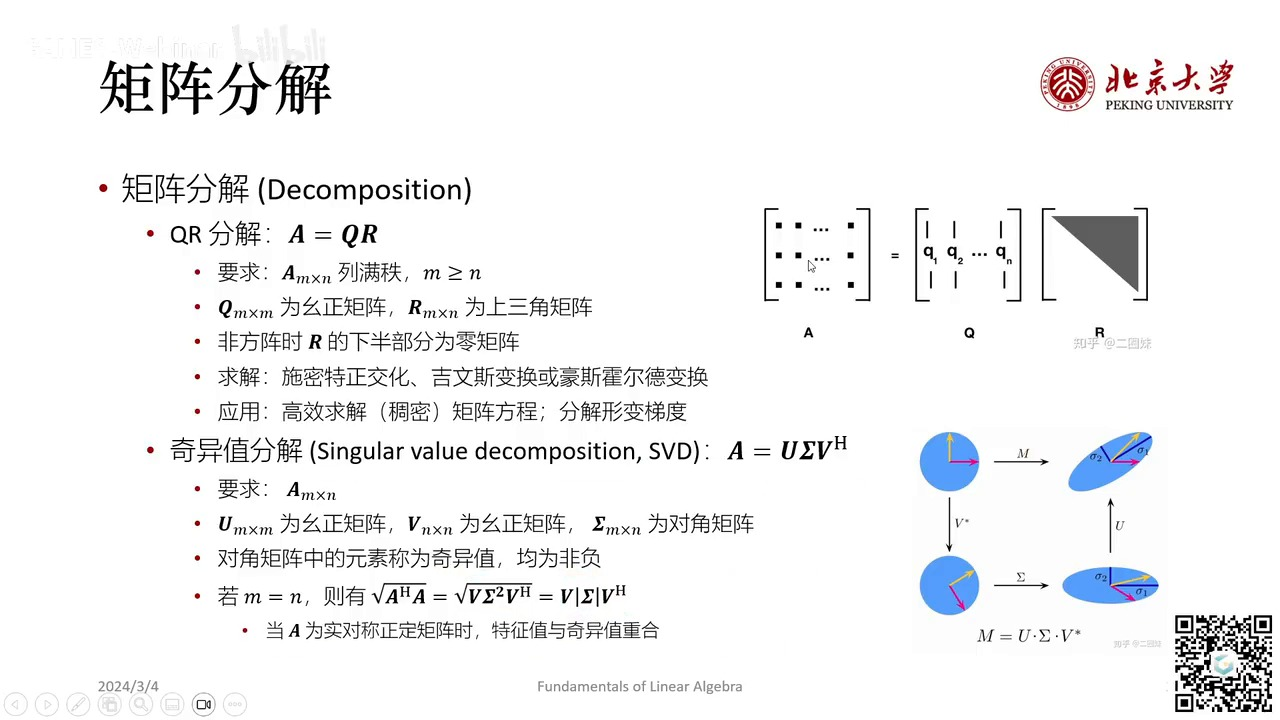
\includegraphics[width=0.92\textwidth]{figures/fig_05_svd_eigen_relation.jpg}
\caption{奇异值与特征值的关系：$\sqrt{\boldsymbol A^{\mathrm H}\boldsymbol A}=\boldsymbol V|\boldsymbol\Sigma|\boldsymbol V^{\mathrm H}$，实对称正定时二者重合\vtag}
\end{figure}
\srcnote{00:33:15--00:33:30}
\end{minipage}


\begin{center}
\begin{tabular}{p{0.12\textwidth}p{0.22\textwidth}p{0.26\textwidth}p{0.28\textwidth}}
\toprule
分解 & 形式 & 要求 & 课件列出的应用 \\
\midrule
PLU & $\boldsymbol A=\boldsymbol P\boldsymbol L\boldsymbol U$ & 方阵 & 高斯消元求解矩阵方程 \\
Cholesky & $\boldsymbol A=\boldsymbol L\boldsymbol L^{\mathrm H}$ & 方阵，正定，实对称/埃尔米特 & 高效求解（稀疏）矩阵方程 \\
QR & $\boldsymbol A=\boldsymbol Q\boldsymbol R$ & 列满秩，$m\ge n$ & 求解（稠密）方程，分解形变梯度 \\
SVD & $\boldsymbol A=\boldsymbol U\boldsymbol\Sigma\boldsymbol V^{\mathrm H}$ & 任意 $m\times n$ 矩阵 & 几何解释、奇异值分析 \\
\bottomrule
\end{tabular}
\end{center}

\subsection{本章小结}

四种分解都在做同一件事：把矩阵换成结构简单的因子。LU 与 Cholesky 把方程变成两次三角回代，Cholesky 还利用了对称正定性；QR 把矩阵拆成正交部分与三角部分，在物理模拟中用来剥离形变中的旋转；SVD 则把任意变换拆成“旋转—缩放—旋转”，奇异值是 $\sqrt{\boldsymbol A^{\mathrm H}\boldsymbol A}$ 的特征值。度量这些矩阵“有多大”，需要下一章的范数。

\section{向量范数：怎样度量长度}

范数是对“长度”的度量。讲者先在向量上定义范数，再推广到矩阵。设 $\boldsymbol x$ 维度为 $n\times1$，常用的向量范数为
\[
\begin{aligned}
L_0:&\ \ \|\boldsymbol x\|_0=\textstyle\sum_{i=1}^{n}[x_i\neq0],\\
L_1:&\ \ \|\boldsymbol x\|_1=\textstyle\sum_{i=1}^{n}|x_i|=|x_1|+|x_2|+\cdots+|x_n|,\\
L_2:&\ \ \|\boldsymbol x\|_2=\sqrt{\textstyle\sum_{i=1}^{n}x_i^2}=(x_1^2+x_2^2+\cdots+x_n^2)^{1/2},\\
L_p:&\ \ \|\boldsymbol x\|_p=(|x_1|^p+|x_2|^p+\cdots+|x_n|^p)^{1/p}\quad(p\ge1),\\
L_\infty:&\ \ \|\boldsymbol x\|_\infty=\max\{|x_1|,|x_2|,\dots,|x_n|\}.
\end{aligned}
\]
\begin{itemize}
\item $x_i$：向量的第 $i$ 个分量；$[x_i\neq0]$：分量非零时取 1，否则取 0；$p$：范数的阶。
\end{itemize}
$L_0$“范数”统计非零元素的个数；$L_2$ 范数又称为欧几里得（Euclidean）或 Frobenius 范数。$L_1$ 与 $L_2$ 都可以写成“各分量绝对值的 $p$ 次幂求和再开 $p$ 次方”，这就是一般的 $L_p$ 范数。讲者用一个比较的例子说明为何 $L_\infty$ 是最大分量：两个数的 $p$ 次幂之和再开 $p$ 次方，当 $p\to\infty$ 时，较大的那个数主导一切，结果趋于最大值。

\noindent\begin{minipage}{\textwidth}
\begin{figure}[H]
\centering
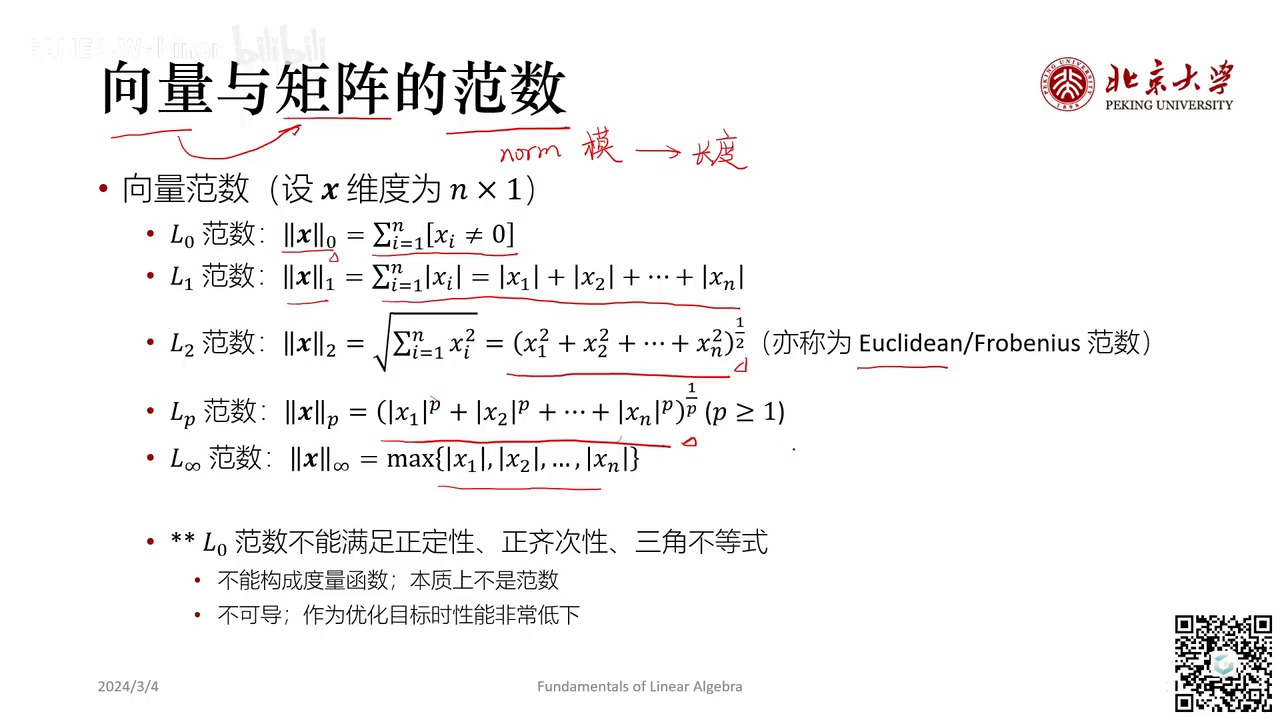
\includegraphics[width=0.92\textwidth]{figures/fig_06_vector_norms.jpg}
\caption{向量范数：$L_0$、$L_1$、$L_2$、$L_p$ 与 $L_\infty$ 的定义\vtag}
\end{figure}
\srcnote{00:35:45--00:36:00}
\end{minipage}


\subsection{为什么 $L_0$ 不是真正的范数}

上一讲回顾过范数必须满足正定性、正齐次性与三角不等式。讲者在手写板上逐条验证：$L_0$ 一条都不满足，所以它本质上不是范数，不能构成度量函数。它在优化中也很难用：作为优化目标时，误差往往写成两个向量之差的“范数”；如果用 $L_0$，它不可导，某个元素从非零变成零时函数值跳变，优化性能非常低下。

\noindent\begin{minipage}{\textwidth}
\begin{figure}[H]
\centering
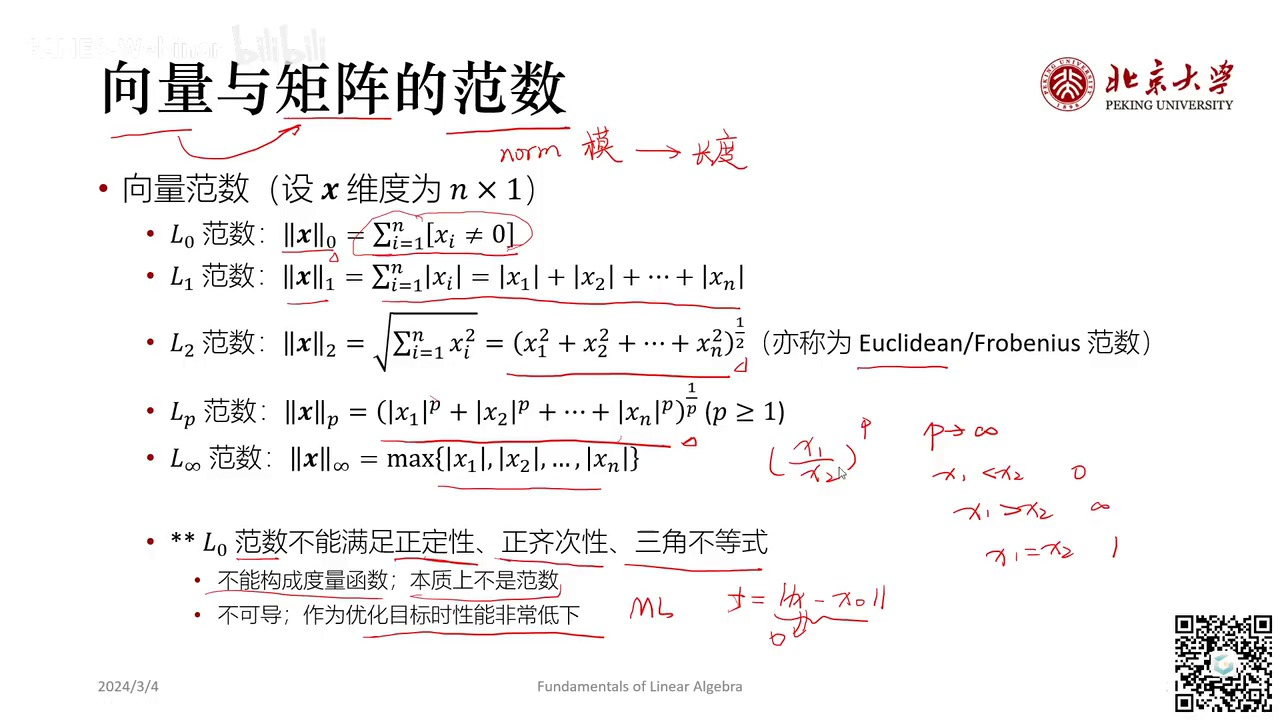
\includegraphics[width=0.92\textwidth]{figures/fig_07_l0_not_norm.jpg}
\caption{手写板上的讨论：$L_0$ 不满足正定性、正齐次性与三角不等式，作为优化目标不可导\vtag}
\end{figure}
\srcnote{00:38:45--00:39:00}
\end{minipage}


\begin{warningbox}{$L_0$ 的名与实}
$L_0$ 统计非零元个数，常被称为“$L_0$ 范数”，但它不满足范数公理，也不可导。需要稀疏性时，实际计算中常用可导或凸的替代量，而不是直接优化 $L_0$。
\end{warningbox}

\subsection{本章小结}

向量范数是一族长度度量，$p$ 越大越偏重最大分量，$L_\infty$ 只看最大分量。$L_0$ 虽然常被叫作范数，但不满足公理，也不适合直接做优化目标。下一章把这套度量推广到矩阵。

\section{矩阵范数：度量一个变换有多“大”}

矩阵范数与向量范数的目的相同：用一个实数表达矩阵的“大小”。设 $\boldsymbol A$ 维度为 $m\times n$。矩阵范数有两种定义思路：一是由向量范数诱导，二是直接基于矩阵元素定义。讲者提醒，两种方式下都会出现“$L_p$ 范数”的叫法，阅读文献时要分清用的是哪一种。

\subsection{诱导范数}

诱导范数（induced norm）定义为
\[
\|\boldsymbol A\|=\max\{\|\boldsymbol A\boldsymbol x\|:\boldsymbol x\in\mathbb K^n,\ \|\boldsymbol x\|=1\}=\max\left\{\frac{\|\boldsymbol A\boldsymbol x\|}{\|\boldsymbol x\|}:\boldsymbol x\in\mathbb K^n,\ \|\boldsymbol x\|\neq0\right\},
\]
\begin{itemize}
\item $\mathbb K^n$：$n$ 维实或复向量空间；$\|\boldsymbol A\boldsymbol x\|$：变换后向量的范数；两种写法分别限定单位向量与任意非零向量。
\end{itemize}
由向量的 $L_p$ 范数可以诱导出矩阵的 $L_p$ 范数。它的几何意义很直接：$\boldsymbol A$ 作为线性变换时，对向量模长的最大放大倍数。诱导范数满足相容性 $\|\boldsymbol A\boldsymbol x\|\le\|\boldsymbol A\|\,\|\boldsymbol x\|$，证明只需一行：
\[
\frac{\|\boldsymbol A\boldsymbol x\|}{\|\boldsymbol x\|}\le\max\left\{\frac{\|\boldsymbol A\boldsymbol x\|}{\|\boldsymbol x\|}:\boldsymbol x\in\mathbb K^n,\ \|\boldsymbol x\|\neq0\right\}=\|\boldsymbol A\| .
\]
\begin{itemize}
\item 左侧：某个特定向量的放大倍数；右侧：所有向量放大倍数的最大值，即诱导范数。
\end{itemize}
三种常用的诱导范数有简单的计算公式：
\[
\|\boldsymbol A\|_1=\max_{1\le j\le n}\sum_{i=1}^{m}|a_{ij}|,\qquad
\|\boldsymbol A\|_2=\sigma_{\max}(\boldsymbol A),\qquad
\|\boldsymbol A\|_\infty=\max_{1\le i\le m}\sum_{j=1}^{n}|a_{ij}|,
\]
\begin{itemize}
\item $\|\boldsymbol A\|_1$：所有列向量的绝对值之和中的最大者（列和范数）；$\|\boldsymbol A\|_\infty$：所有行向量的绝对值之和中的最大者（行和范数）；$\sigma_{\max}$：$\boldsymbol A$ 的最大奇异值。
\end{itemize}
$\|\boldsymbol A\|_2$ 又称为谱范数，课件把“如何证明”留作作业。讲者指出 $\|\boldsymbol A\|_1$ 与 $\|\boldsymbol A\|_\infty$ 恰好对应：一个看列，一个看行。

\noindent\begin{minipage}{\textwidth}
\begin{figure}[H]
\centering
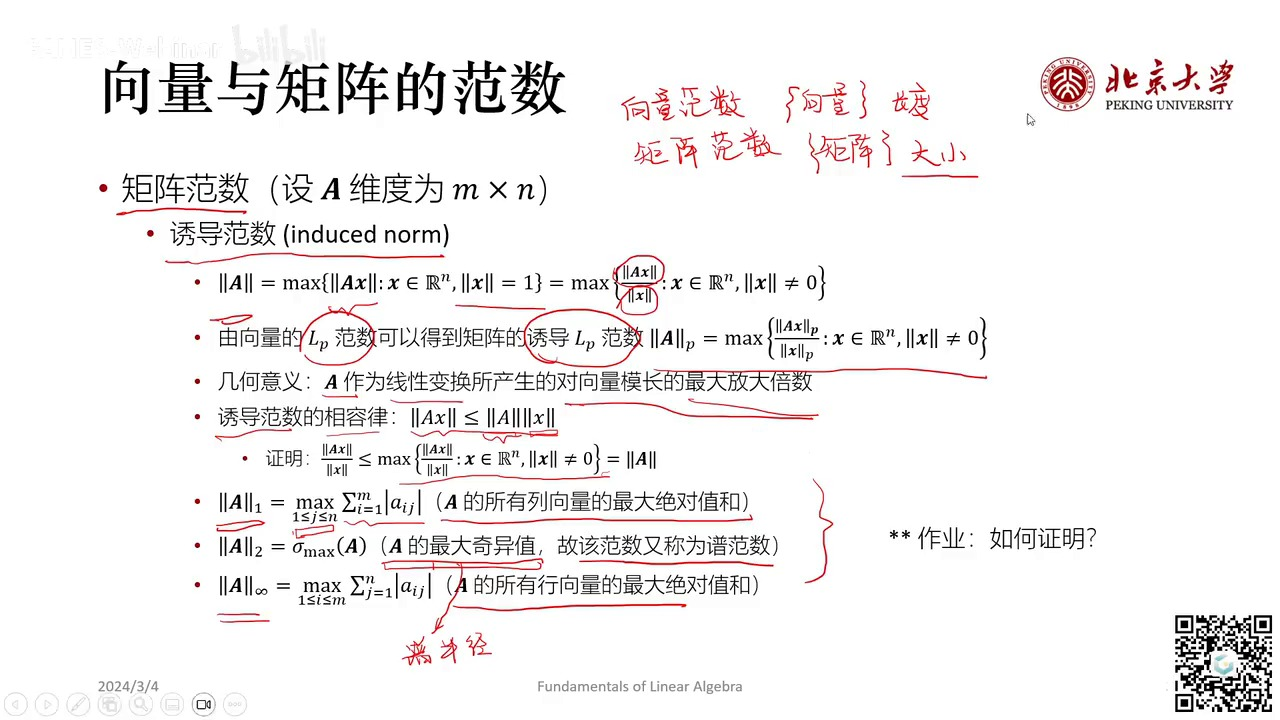
\includegraphics[width=0.92\textwidth]{figures/fig_08_induced_norm.jpg}
\caption{诱导范数：最大放大倍数、相容性及其证明，以及 $\|\boldsymbol A\|_1$、$\|\boldsymbol A\|_2$、$\|\boldsymbol A\|_\infty$ 的计算\vtag}
\end{figure}
\srcnote{00:43:30--00:43:45}
\end{minipage}


\subsection{元素形式范数}

元素形式范数（entrywise norm）把矩阵按元素展开，当作一个长向量来使用向量的 $L_p$ 范数：
\[
\|\boldsymbol A\|_1=\sum_{i=1}^{m}\sum_{j=1}^{n}|a_{ij}|,\qquad
\|\boldsymbol A\|_F=\Big(\sum_{i=1}^{m}\sum_{j=1}^{n}a_{ij}^2\Big)^{1/2}=\operatorname{tr}\boldsymbol A^{\mathsf T}\boldsymbol A,\qquad
\|\boldsymbol A\|_{\max}=\max_{i,j}|a_{ij}| .
\]
\begin{itemize}
\item $\|\cdot\|_1$：和范数（元素 $L_1$）；$\|\cdot\|_F$：Frobenius 范数，也叫 Euclidean、Schur 或元素 $L_2$ 范数，是每个元素平方求和再开根号；$\|\cdot\|_{\max}$：最大范数（元素 $L_\infty$）。
\end{itemize}
\begin{warningbox}{Frobenius 范数的迹表示}
课件把 Frobenius 范数写成 $\operatorname{tr}\boldsymbol A^{\mathsf T}\boldsymbol A$。讲义作者注：严格地说 $\|\boldsymbol A\|_F^2=\operatorname{tr}\boldsymbol A^{\mathsf T}\boldsymbol A$，即 $\|\boldsymbol A\|_F=\sqrt{\operatorname{tr}\boldsymbol A^{\mathsf T}\boldsymbol A}$，因为 $\boldsymbol A^{\mathsf T}\boldsymbol A$ 的对角元恰好是各列的平方和。
\end{warningbox}

\subsection{Schatten 范数}

沙滕（Schatten）范数是一种不随幺正变换而改变的范数。做法是利用“幺正变换不改变奇异值”：把范数定义在奇异值上，
\[
\|\boldsymbol A\|_p=\Big(\sum_{i=1}^{\min\{m,n\}}\sigma_i^p\Big)^{1/p},
\]
\begin{itemize}
\item $\sigma_i$：$\boldsymbol A$ 的第 $i$ 个奇异值；$p$：阶数。
\end{itemize}
几个特例：$\|\boldsymbol A\|_1$ 是奇异值之和，称为核范数（nuclear norm）；$\|\boldsymbol A\|_2=\|\boldsymbol A\|_F$；$\|\boldsymbol A\|_\infty$ 等价于谱范数。讲者的总结是：对奇异值组成的向量求 $L_1$，就是矩阵的 Schatten-1 范数；求 $L_2$，就是 Schatten-2 范数，依此类推。这些性质都不难证明。

\noindent\begin{minipage}{\textwidth}
\begin{figure}[H]
\centering
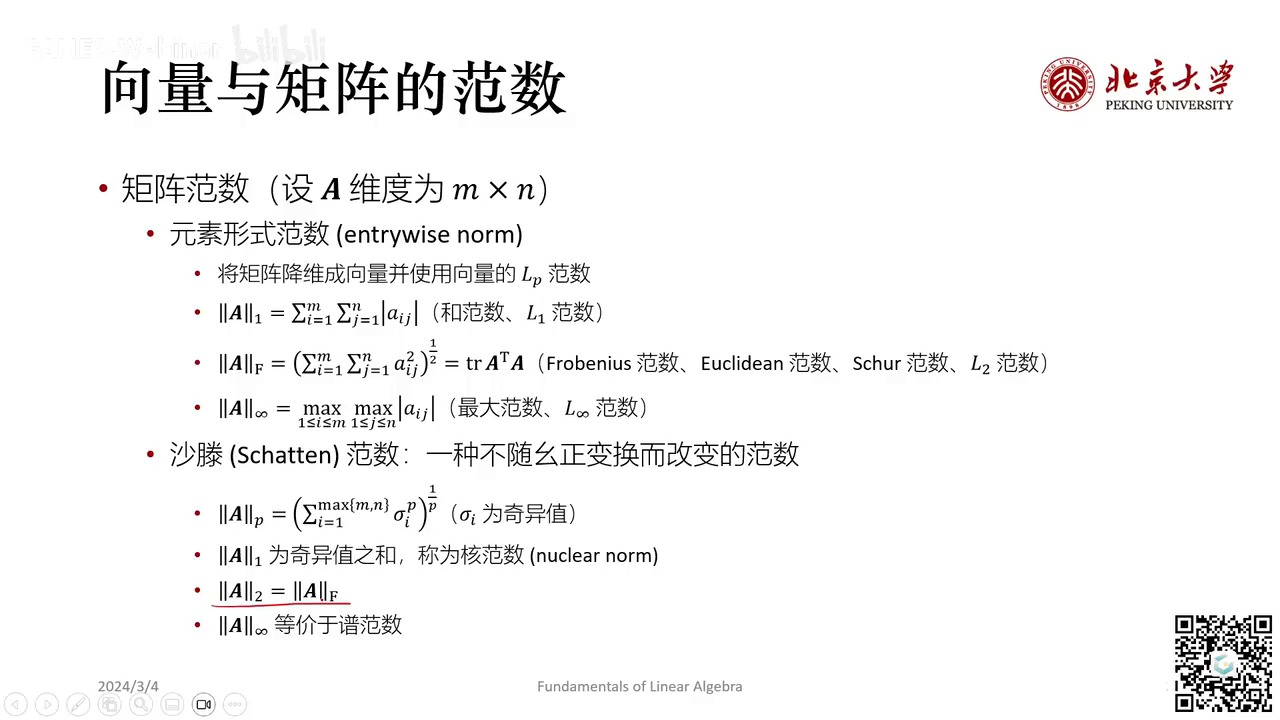
\includegraphics[width=0.92\textwidth]{figures/fig_09_entrywise_schatten.jpg}
\caption{元素形式范数与 Schatten 范数：前者把矩阵当长向量，后者把范数定义在奇异值上\vtag}
\end{figure}
\srcnote{00:47:30--00:47:45}
\end{minipage}


\begin{knowledgebox}{三类矩阵范数的对照}
\begin{itemize}
\item 诱导范数衡量“变换对向量的最大放大倍数”，$\|\boldsymbol A\|_2$ 是最大奇异值；
\item 元素形式范数把矩阵当作 $mn$ 维向量，Frobenius 范数最常用；
\item Schatten 范数对奇异值向量取 $L_p$，因此在幺正变换下不变；Schatten-2 等于 Frobenius，Schatten-$\infty$ 等于谱范数。
\end{itemize}
\end{knowledgebox}

\subsection{本章小结}

矩阵范数有三条定义路线：通过最大放大倍数诱导、按元素展开、作用在奇异值上。它们在名称上都可能叫“$L_p$”，含义却不同。范数给了我们衡量残差的尺子；要让残差最小，还需要对矩阵求导。

\section{矩阵求导：布局与基本公式}

\subsection{为什么图形学需要矩阵求导}

倪星宇结合自己的研究方向，总结了矩阵求导在图形学中的两类应用（他强调实际应用远不止这两点）。

\paragraph{伴随方法。}伴随方法要求物理量相对于初始参数的导数，相当于深度学习中求输出相对于输入的导数。讲者类比高中物理的抛体问题：给定初始角度 $\theta$ 与初速度 $v_0$，求落点；反过来，若要命中某个位置，就要知道落点对 $\theta$、$v_0$ 的导数。真实问题中初始参数远不止两个，得到的结果也不只是一个落点，于是需要矩阵形式的求导。物理模拟往往是一长串时间步的迭代，每一步都是矩阵运算；要把最终结果对初始参数的敏感度一路传回去，就要在每一步对向量、矩阵求导，并按链式法则组合起来。这与深度学习中的反向传播是同一类问题。

\paragraph{软体仿真中的应力张量。}给定势能函数求应力张量是课程作业的一部分。形变梯度 $\boldsymbol F$ 是 $3\times3$ 矩阵，弹性势能密度 $\psi$ 是标量，第一类 Piola--Kirchhoff 应力为 $\boldsymbol P=\partial\psi/\partial\boldsymbol F$；由它可以得到柯西应力张量，进而算出力。这里就是一个“标量对矩阵求导”的过程：自变量 $\boldsymbol F$ 是矩阵，因变量 $\psi$ 是标量，结果 $\boldsymbol P$ 与 $\boldsymbol F$ 同为 $3\times3$ 矩阵。不同的材料模型给出不同的 $\psi(\boldsymbol F)$，例如其中常含有 $\operatorname{tr}(\boldsymbol F^{\mathsf T}\boldsymbol F)$ 或 $\det\boldsymbol F$ 这样的项；后文推出的迹与行列式的导数，正好用来计算这类应力。

\noindent\begin{minipage}{\textwidth}
\begin{figure}[H]
\centering
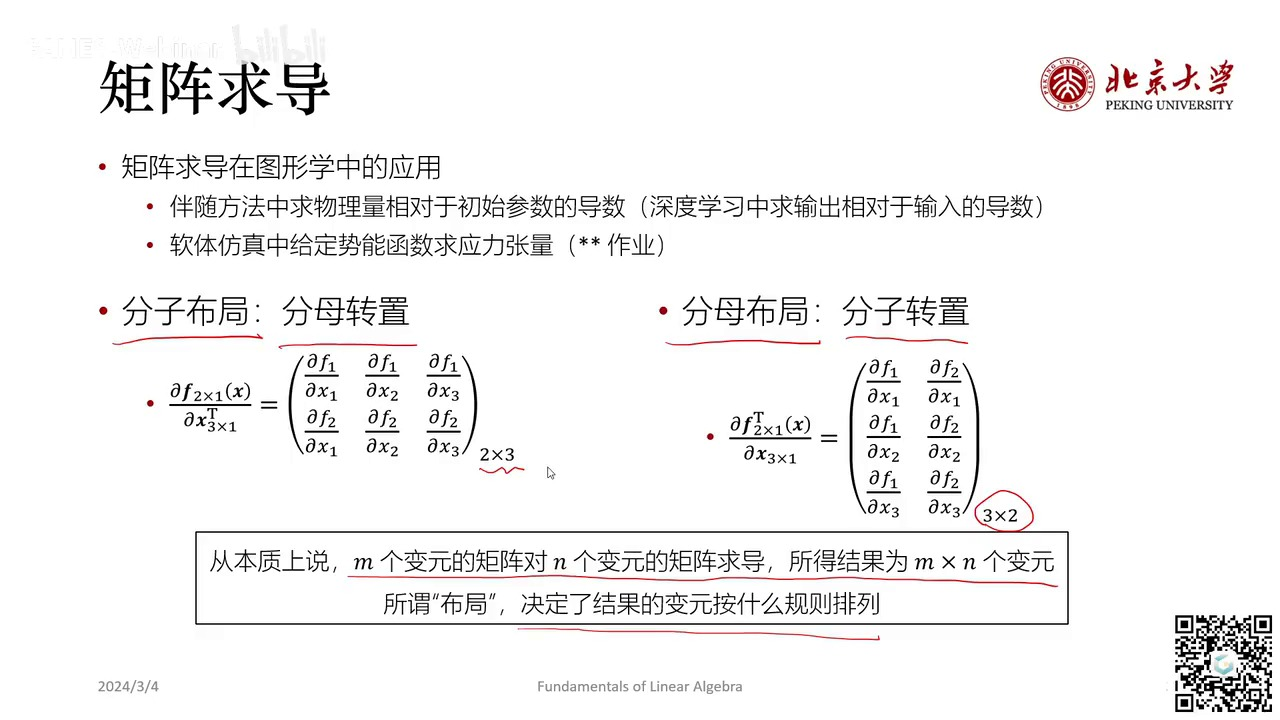
\includegraphics[width=0.92\textwidth]{figures/fig_10_derivative_layout.jpg}
\caption{矩阵求导的两类应用，以及分子布局与分母布局\vtag}
\end{figure}
\srcnote{00:53:00--00:53:15}
\end{minipage}


\subsection{分子布局与分母布局}

矩阵求导有两种布局。分子布局下分母转置：
\[
\frac{\partial\boldsymbol f_{2\times1}(\boldsymbol x)}{\partial\boldsymbol x^{\mathsf T}_{3\times1}}=
\begin{pmatrix}
\dfrac{\partial f_1}{\partial x_1}&\dfrac{\partial f_1}{\partial x_2}&\dfrac{\partial f_1}{\partial x_3}\\[2mm]
\dfrac{\partial f_2}{\partial x_1}&\dfrac{\partial f_2}{\partial x_2}&\dfrac{\partial f_2}{\partial x_3}
\end{pmatrix}_{2\times3};
\]
\begin{itemize}
\item $\boldsymbol f$：$2$ 维向量函数；$\boldsymbol x$：$3$ 维自变量；结果的行对应函数分量、列对应自变量分量。
\end{itemize}
分母布局下分子转置：
\[
\frac{\partial\boldsymbol f^{\mathsf T}_{2\times1}(\boldsymbol x)}{\partial\boldsymbol x_{3\times1}}=
\begin{pmatrix}
\dfrac{\partial f_1}{\partial x_1}&\dfrac{\partial f_2}{\partial x_1}\\[2mm]
\dfrac{\partial f_1}{\partial x_2}&\dfrac{\partial f_2}{\partial x_2}\\[2mm]
\dfrac{\partial f_1}{\partial x_3}&\dfrac{\partial f_2}{\partial x_3}
\end{pmatrix}_{3\times2}.
\]
\begin{itemize}
\item 结果的行对应自变量分量、列对应函数分量，与分子布局互为转置。
\end{itemize}
讲者给了一个记忆口诀：“谁转置就不是谁的布局”，分母转置是分子布局，分子转置是分母布局。从本质上说，$m$ 个变元的矩阵对 $n$ 个变元的矩阵求导，结果是 $m\times n$ 个变元，所谓“布局”只决定了这些结果按什么规则排列。两种布局混用会导致矩阵乘法不相容，所以推导时必须固定一种。

\begin{knowledgebox}{布局口诀}
“谁转置就不是谁的布局”：$\partial\boldsymbol f/\partial\boldsymbol x^{\mathsf T}$ 是分子布局（结果的行随 $\boldsymbol f$），$\partial\boldsymbol f^{\mathsf T}/\partial\boldsymbol x$ 是分母布局（结果的行随 $\boldsymbol x$）。本讲后面的“微分—迹”法则使用分子布局。
\end{knowledgebox}

\subsection{向量变元的实值标量函数}

设 $\boldsymbol x_{n\times1}=(x_1,\dots,x_n)^{\mathsf T}$，梯度定义为
\[
\nabla_{\boldsymbol x}f(\boldsymbol x)=\frac{\partial f(\boldsymbol x)}{\partial\boldsymbol x_{n\times1}}=\left(\frac{\partial f}{\partial x_1},\frac{\partial f}{\partial x_2},\dots,\frac{\partial f}{\partial x_n}\right)^{\mathsf T},
\]
\begin{itemize}
\item $f$：实值标量函数；梯度：对每个分量求偏导后组装成列向量。
\end{itemize}
运算法则与单变量求导一致：常数的导数为零向量 $\boldsymbol 0_{n\times1}$；线性法则 $\partial(c_1f+c_2g)/\partial\boldsymbol x=c_1\partial f/\partial\boldsymbol x+c_2\partial g/\partial\boldsymbol x$；乘积法则 $\partial(fg)/\partial\boldsymbol x=(\partial f/\partial\boldsymbol x)g+f(\partial g/\partial\boldsymbol x)$，讲者特别说明这里 $f,g$ 是实数，所以乘积是“列向量乘实数加实数乘列向量”；商法则同理。常用公式（$\boldsymbol a_{n\times1},\boldsymbol b_{n\times1}$ 为常数向量，$\boldsymbol A_{n\times n}$ 为常数矩阵）为
\[
\frac{\partial(\boldsymbol a^{\mathsf T}\boldsymbol x)}{\partial\boldsymbol x}=\frac{\partial(\boldsymbol x^{\mathsf T}\boldsymbol a)}{\partial\boldsymbol x}=\boldsymbol a,\quad
\frac{\partial(\boldsymbol x^{\mathsf T}\boldsymbol x)}{\partial\boldsymbol x}=2\boldsymbol x,\quad
\frac{\partial(\boldsymbol x^{\mathsf T}\boldsymbol A\boldsymbol x)}{\partial\boldsymbol x}=\boldsymbol A\boldsymbol x+\boldsymbol A^{\mathsf T}\boldsymbol x,\quad
\frac{\partial(\boldsymbol a^{\mathsf T}\boldsymbol x\boldsymbol x^{\mathsf T}\boldsymbol b)}{\partial\boldsymbol x}=\boldsymbol a\boldsymbol b^{\mathsf T}\boldsymbol x+\boldsymbol b\boldsymbol a^{\mathsf T}\boldsymbol x .
\]
\begin{itemize}
\item $\boldsymbol a^{\mathsf T}\boldsymbol x$：内积，导数是“不变的那个向量”$\boldsymbol a$；$\boldsymbol x^{\mathsf T}\boldsymbol A\boldsymbol x$：二次型，$\boldsymbol A$ 对称时导数为 $2\boldsymbol A\boldsymbol x$。
\end{itemize}
讲者说，第一条可以理解为对内积求导得到“另一个不变元”，第二条可以看成第三条在 $\boldsymbol A=\boldsymbol E$ 时的特例，验证都很容易。

\noindent\begin{minipage}{\textwidth}
\begin{figure}[H]
\centering
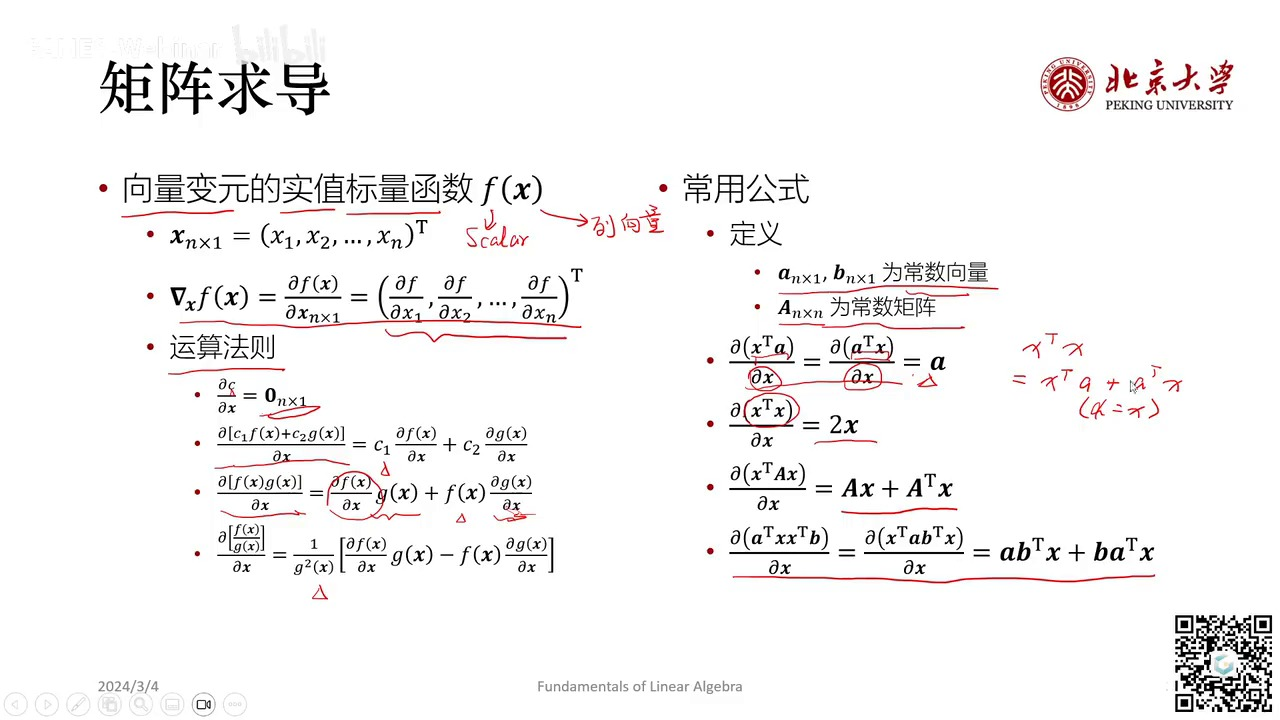
\includegraphics[width=0.92\textwidth]{figures/fig_11_vector_derivative.jpg}
\caption{向量变元的实值标量函数：梯度定义、运算法则与常用公式\vtag}
\end{figure}
\srcnote{00:57:45--00:58:00}
\end{minipage}


\subsection{矩阵变元的实值标量函数}

当自变量变为矩阵 $\boldsymbol X_{m\times n}=(x_{ij})$ 时，
\[
\nabla_{\boldsymbol X}f(\boldsymbol X)=\frac{\partial f(\boldsymbol X)}{\partial\boldsymbol X_{m\times n}}=
\begin{pmatrix}\dfrac{\partial f}{\partial x_{11}}&\cdots&\dfrac{\partial f}{\partial x_{1n}}\\ \vdots&\ddots&\vdots\\ \dfrac{\partial f}{\partial x_{m1}}&\cdots&\dfrac{\partial f}{\partial x_{mn}}\end{pmatrix},
\]
\begin{itemize}
\item $x_{ij}$：矩阵变元的元素；结果与 $\boldsymbol X$ 同形。
\end{itemize}
运算法则（线性、乘积、商）与向量情形相同。常用公式（$\boldsymbol a_{m\times1},\boldsymbol b_{n\times1}$ 为常数向量）为
\[
\begin{gathered}
\frac{\partial(\boldsymbol a^{\mathsf T}\boldsymbol X\boldsymbol b)}{\partial\boldsymbol X}=\boldsymbol a\boldsymbol b^{\mathsf T},\quad
\frac{\partial(\boldsymbol a^{\mathsf T}\boldsymbol X^{\mathsf T}\boldsymbol b)}{\partial\boldsymbol X}=\boldsymbol b\boldsymbol a^{\mathsf T},\\
\frac{\partial(\boldsymbol a^{\mathsf T}\boldsymbol X\boldsymbol X^{\mathsf T}\boldsymbol b)}{\partial\boldsymbol X}=\boldsymbol a\boldsymbol b^{\mathsf T}\boldsymbol X+\boldsymbol b\boldsymbol a^{\mathsf T}\boldsymbol X,\quad
\frac{\partial(\boldsymbol a^{\mathsf T}\boldsymbol X^{\mathsf T}\boldsymbol X\boldsymbol b)}{\partial\boldsymbol X}=\boldsymbol X\boldsymbol b\boldsymbol a^{\mathsf T}+\boldsymbol X\boldsymbol a\boldsymbol b^{\mathsf T}.
\end{gathered}
\]
\begin{itemize}
\item 第二式由第一式整体转置得到；第三、四式需要用到乘积法则，第三四两式的 $\boldsymbol a,\boldsymbol b$ 维度课件均写为 $m\times1$。
\end{itemize}

\noindent\begin{minipage}{\textwidth}
\begin{figure}[H]
\centering
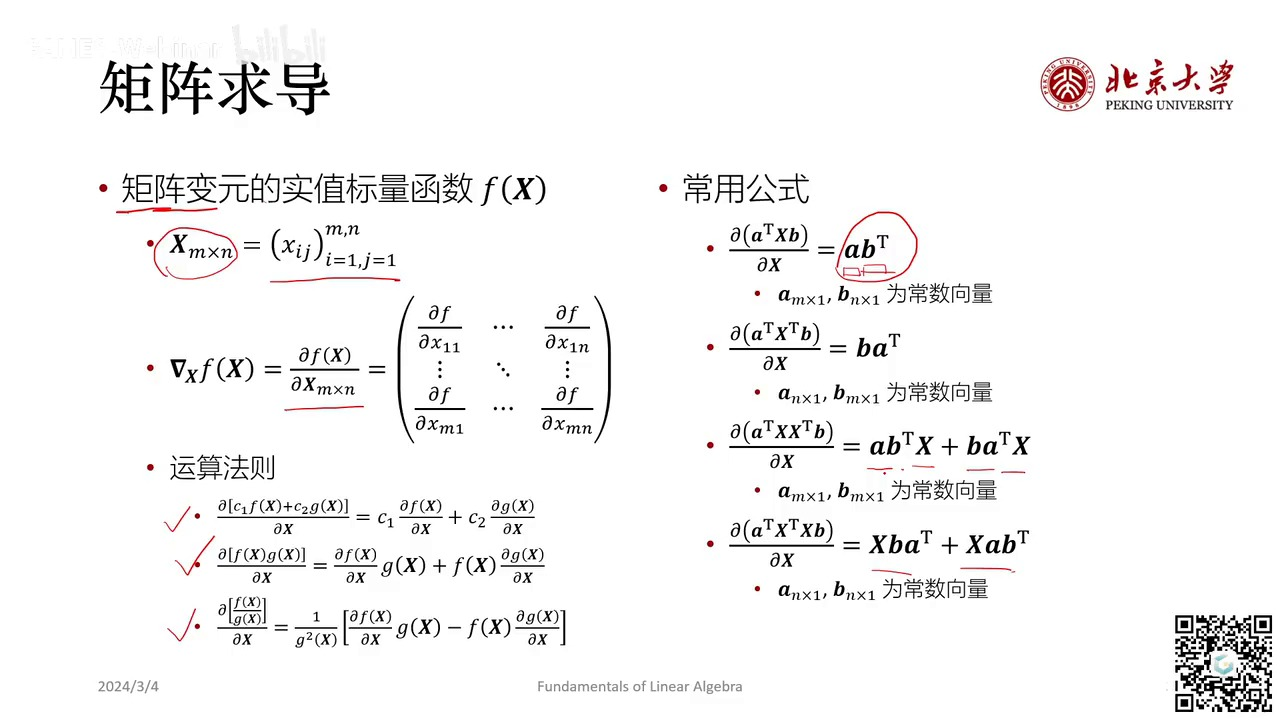
\includegraphics[width=0.92\textwidth]{figures/fig_12_matrix_derivative.jpg}
\caption{矩阵变元的实值标量函数：梯度定义与常用公式\vtag}
\end{figure}
\srcnote{01:00:45--01:01:00}
\end{minipage}


\subsection{本章小结}

矩阵求导首先是一个排列约定：分子布局与分母布局互为转置，推导中必须统一。向量与矩阵变元的标量函数，其导数与自变量同形，法则与一元求导相同。但直接按定义逐元素求导很繁琐，下一章介绍更实用的“微分—迹”方法。

\section{矩阵微分与“微分—迹”技巧}

\subsection{矩阵函数的微分}

讲者解释为什么要讲矩阵函数的微分：它能以更简便的方式计算前面那些导数。对向量变元的实值标量函数，
\[
\mathrm df(\boldsymbol x)=\left(\frac{\partial f}{\partial x_1},\dots,\frac{\partial f}{\partial x_n}\right)\begin{pmatrix}\mathrm dx_1\\ \vdots\\ \mathrm dx_n\end{pmatrix}=\operatorname{tr}\left[\left(\frac{\partial f}{\partial x_1},\dots,\frac{\partial f}{\partial x_n}\right)\begin{pmatrix}\mathrm dx_1\\ \vdots\\ \mathrm dx_n\end{pmatrix}\right],
\]
\begin{itemize}
\item $\mathrm dx_i$：自变量分量的微分；加上迹不改变结果，因为 $1\times1$ 矩阵的迹就是它唯一的元素。
\end{itemize}
对矩阵变元的实值标量函数，
\[
\mathrm df(\boldsymbol X)=\operatorname{tr}\left[\begin{pmatrix}\dfrac{\partial f}{\partial x_{11}}&\cdots&\dfrac{\partial f}{\partial x_{m1}}\\ \vdots&\ddots&\vdots\\ \dfrac{\partial f}{\partial x_{1n}}&\cdots&\dfrac{\partial f}{\partial x_{mn}}\end{pmatrix}_{n\times m}
\begin{pmatrix}\mathrm dx_{11}&\cdots&\mathrm dx_{1n}\\ \vdots&\ddots&\vdots\\ \mathrm dx_{m1}&\cdots&\mathrm dx_{mn}\end{pmatrix}_{m\times n}\right],
\]
\begin{itemize}
\item 左因子是 $\partial f/\partial\boldsymbol X^{\mathsf T}$（分子布局，$n\times m$）；右因子是 $\mathrm d\boldsymbol X$；乘积取迹后正好是 $\sum_{ij}(\partial f/\partial x_{ij})\mathrm dx_{ij}$。
\end{itemize}

\noindent\begin{minipage}{\textwidth}
\begin{figure}[H]
\centering
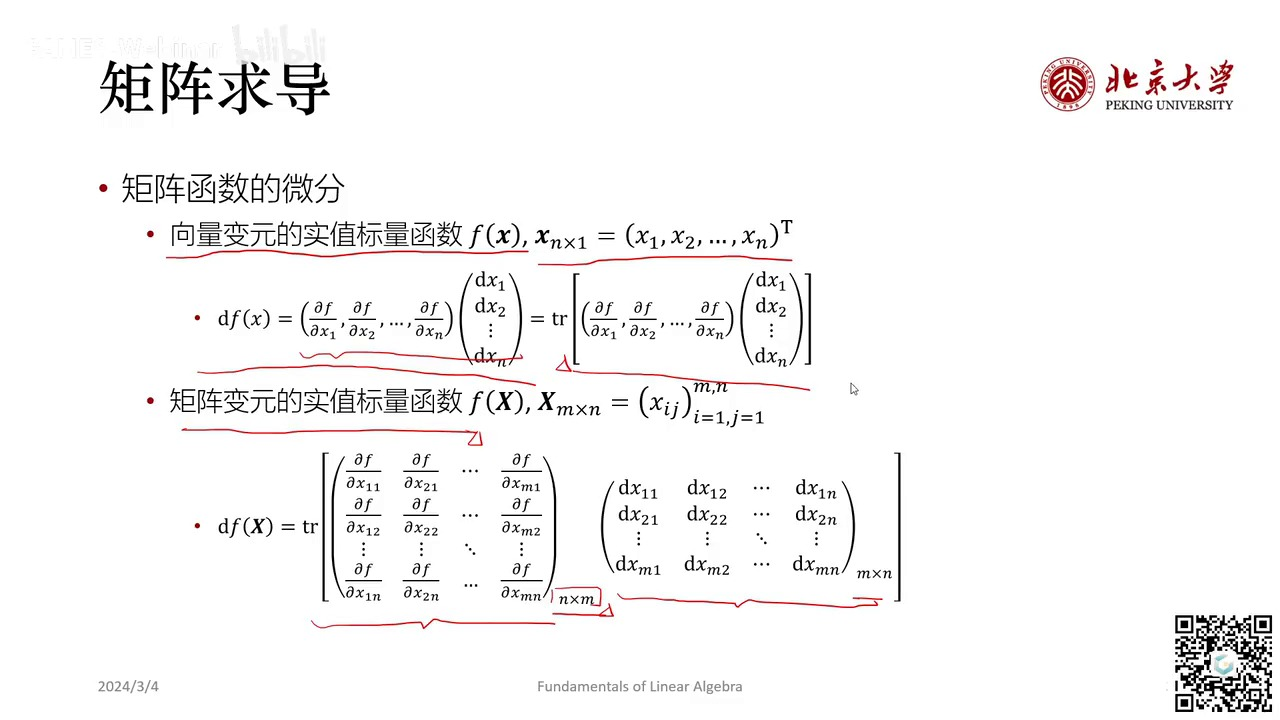
\includegraphics[width=0.92\textwidth]{figures/fig_13_matrix_differential.jpg}
\caption{矩阵函数的微分：向量变元与矩阵变元的实值标量函数，微分都可以写成迹的形式\vtag}
\end{figure}
\srcnote{01:03:00--01:03:15}
\end{minipage}


矩阵变元的实矩阵函数 $\boldsymbol F_{p\times q}(\boldsymbol X)$ 的微分，就是对每个元素求微分后排成同形矩阵。讲者强调：微分不可能改变函数的形状。函数在两个非常接近的自变量处取值相减，结果与函数值同形；若 $f$ 是标量，$\mathrm df$ 是标量，若 $\boldsymbol F$ 是矩阵，$\mathrm d\boldsymbol F$ 是同形矩阵。其法则为
\[
\begin{aligned}
&\mathrm d\boldsymbol A_{m\times n}=\boldsymbol 0_{m\times n},\qquad
\mathrm d\big(c_1\boldsymbol F(\boldsymbol X)+c_2\boldsymbol G(\boldsymbol X)\big)=c_1\mathrm d\boldsymbol F(\boldsymbol X)+c_2\mathrm d\boldsymbol G(\boldsymbol X),\\
&\mathrm d[\boldsymbol F(\boldsymbol X)\boldsymbol G(\boldsymbol X)]=[\mathrm d\boldsymbol F(\boldsymbol X)]\boldsymbol G(\boldsymbol X)+\boldsymbol F(\boldsymbol X)[\mathrm d\boldsymbol G(\boldsymbol X)],\qquad
\mathrm d\boldsymbol F^{\mathsf T}_{p\times q}(\boldsymbol X)=[\mathrm d\boldsymbol F_{p\times q}(\boldsymbol X)]^{\mathsf T}.
\end{aligned}
\]
\begin{itemize}
\item $\boldsymbol A$：常数矩阵；$c_1,c_2$：常数；$\boldsymbol F,\boldsymbol G$：矩阵函数。
\end{itemize}
乘积法则可推广到三个因子：$\mathrm d[\boldsymbol F\boldsymbol G\boldsymbol H]=[\mathrm d\boldsymbol F]\boldsymbol G\boldsymbol H+\boldsymbol F[\mathrm d\boldsymbol G]\boldsymbol H+\boldsymbol F\boldsymbol G[\mathrm d\boldsymbol H]$。讲者反复提醒：乘子顺序不能交换，永远是先 $\boldsymbol F$ 再 $\boldsymbol G$ 再 $\boldsymbol H$。

\noindent\begin{minipage}{\textwidth}
\begin{figure}[H]
\centering
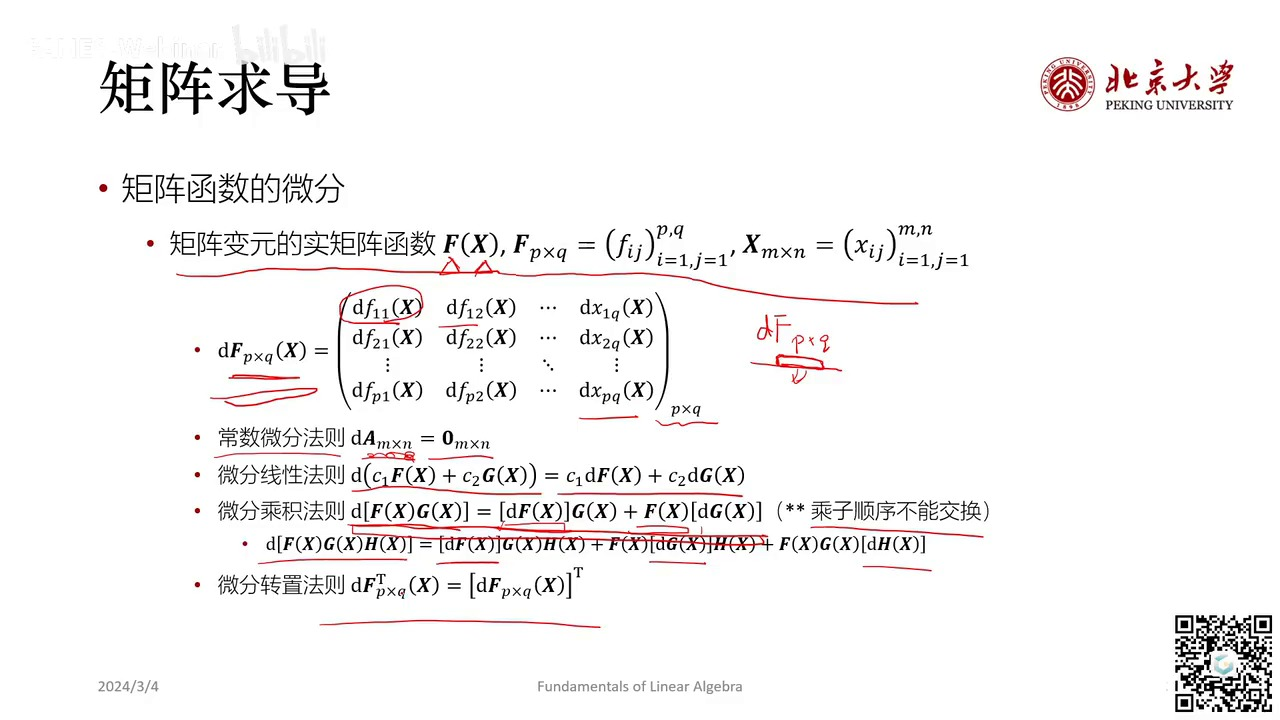
\includegraphics[width=0.92\textwidth]{figures/fig_14_differential_rules.jpg}
\caption{矩阵变元的实矩阵函数的微分法则：常数、线性、乘积与转置，乘子顺序不能交换\vtag}
\end{figure}
\srcnote{01:07:15--01:07:30}
\end{minipage}


\begin{warningbox}{乘积法则的顺序}
矩阵乘法不可交换，所以 $\mathrm d(\boldsymbol F\boldsymbol G)\neq\boldsymbol G\,\mathrm d\boldsymbol F+\dots$。每一项只把微分算子放到某一个因子上，其余因子保持原来的左右位置。
\end{warningbox}

\subsection{利用矩阵微分求导}

核心结论是：若能把标量函数的微分整理成
\[
\mathrm df(\boldsymbol X)=\operatorname{tr}\left[\frac{\partial f(\boldsymbol X)}{\partial\boldsymbol X^{\mathsf T}}\,\mathrm d\boldsymbol X\right],
\]
\begin{itemize}
\item $\partial f/\partial\boldsymbol X^{\mathsf T}$：分子布局下的导数；$\mathrm d\boldsymbol X$：自变量的微分，
\end{itemize}
那么迹里面 $\mathrm d\boldsymbol X$ 左边的那个矩阵就是所求的导数。配合常数矩阵的微分 $\mathrm d(\boldsymbol A\boldsymbol X\boldsymbol B)=\boldsymbol A(\mathrm d\boldsymbol X)\boldsymbol B$（$\boldsymbol A_{p\times m},\boldsymbol B_{n\times q}$ 为常数矩阵）和迹的轮换性，许多导数可以“一步一步写出来”。讲者的做法是：先求函数的微分，再看它与自变量微分之间的关系，剩下的就是导数。

\begin{importantbox}{微分—迹法则}
求标量函数对矩阵的导数：(1) 对函数取微分，利用乘积法则展开；(2) 把标量写成 $1\times1$ 矩阵的迹；(3) 用 $\operatorname{tr}(\boldsymbol A\boldsymbol B)=\operatorname{tr}(\boldsymbol B\boldsymbol A)$ 与 $\operatorname{tr}\boldsymbol A=\operatorname{tr}\boldsymbol A^{\mathsf T}$ 把 $\mathrm d\boldsymbol X$ 移到最右边；(4) 读出 $\mathrm d\boldsymbol X$ 左侧的矩阵，即 $\partial f/\partial\boldsymbol X^{\mathsf T}$。
\end{importantbox}

\noindent\begin{minipage}{\textwidth}
\begin{figure}[H]
\centering
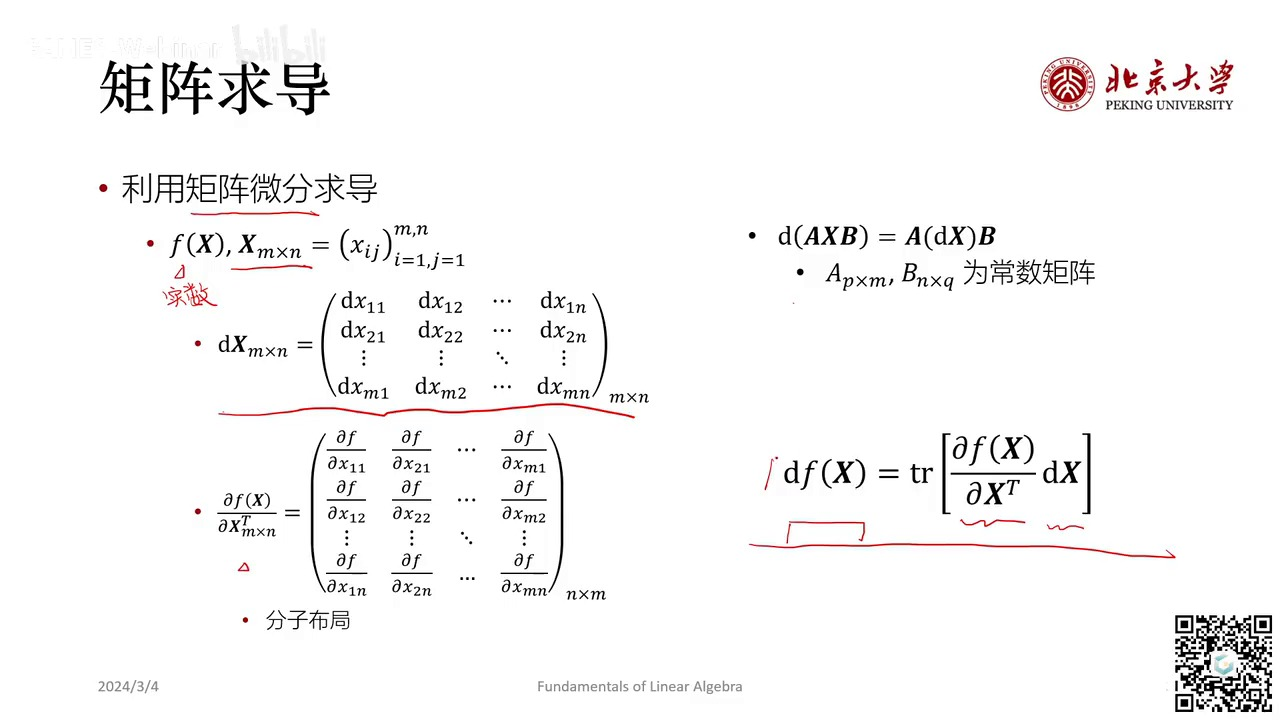
\includegraphics[width=0.92\textwidth]{figures/fig_15_trace_trick.jpg}
\caption{利用矩阵微分求导：$\mathrm df(\boldsymbol X)=\operatorname{tr}[\partial f/\partial\boldsymbol X^{\mathsf T}\,\mathrm d\boldsymbol X]$\vtag}
\end{figure}
\srcnote{01:11:15--01:11:30}
\end{minipage}


\subsection{行列式与逆矩阵的导数}

第一个例子是行列式。按第 $i$ 行展开，$|\boldsymbol X|=x_{i1}A_{i1}+x_{i2}A_{i2}+\cdots+x_{in}A_{in}$（对任意 $i$，$A_{ij}$ 为代数余子式），因此 $\partial|\boldsymbol X|/\partial x_{ij}=A_{ij}$。把所有代数余子式排成矩阵，就得到
\[
\frac{\partial|\boldsymbol X|}{\partial\boldsymbol X^{\mathsf T}}=\boldsymbol X^{*}=\begin{pmatrix}A_{11}&A_{12}&\cdots&A_{1n}\\ \vdots&&\ddots&\vdots\\ A_{n1}&A_{n2}&\cdots&A_{nn}\end{pmatrix}^{\mathsf T},\qquad \boldsymbol X^{-1}=\frac{\boldsymbol X^{*}}{|\boldsymbol X|},
\]
\begin{itemize}
\item $\boldsymbol X^{*}$：伴随矩阵；第二式是线性代数中伴随矩阵与逆矩阵的关系。
\end{itemize}
代入微分—迹法则：$\mathrm d|\boldsymbol X|=\operatorname{tr}(|\boldsymbol X|\boldsymbol X^{-1}\mathrm d\boldsymbol X)=|\boldsymbol X|\operatorname{tr}(\boldsymbol X^{-1}\mathrm d\boldsymbol X)$。

第二个例子是逆矩阵的微分。讲者说这种形式会经常遇到，因为我们定义的标量函数里常常用到的不是 $\boldsymbol X$ 本身，而是它的逆。从 $\boldsymbol X\boldsymbol X^{-1}=\boldsymbol E$ 两边取微分：
\[
(\mathrm d\boldsymbol X)\boldsymbol X^{-1}+\boldsymbol X\,\mathrm d(\boldsymbol X^{-1})=\boldsymbol 0\ \Rightarrow\ \mathrm d(\boldsymbol X^{-1})=-\boldsymbol X^{-1}(\mathrm d\boldsymbol X)\boldsymbol X^{-1}.
\]
\begin{itemize}
\item $\boldsymbol E$：单位矩阵，其微分为零；第二步左乘 $\boldsymbol X^{-1}$ 后移项。
\end{itemize}

\noindent\begin{minipage}{\textwidth}
\begin{figure}[H]
\centering
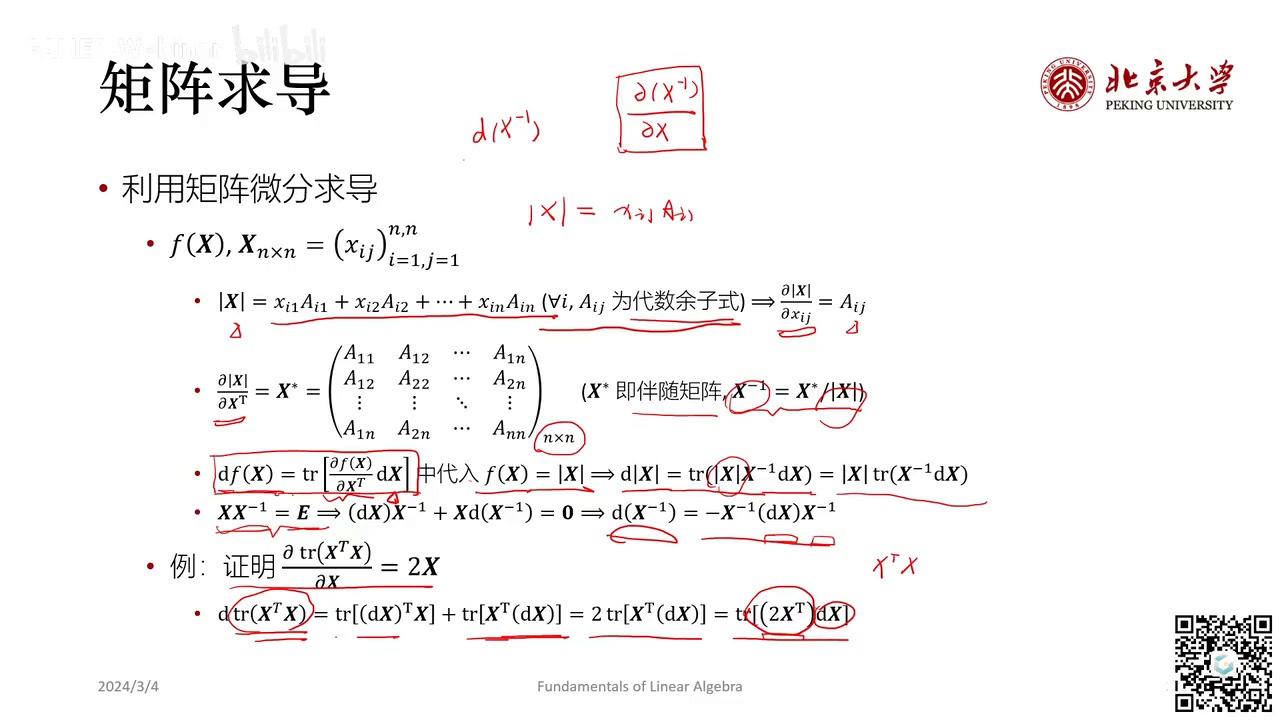
\includegraphics[width=0.92\textwidth]{figures/fig_16_det_inverse_derivative.jpg}
\caption{利用矩阵微分求行列式与逆矩阵的导数，以及 $\partial\operatorname{tr}(\boldsymbol X^{\mathsf T}\boldsymbol X)/\partial\boldsymbol X=2\boldsymbol X$ 的证明\vtag}
\end{figure}
\srcnote{01:19:00--01:19:15}
\end{minipage}


作为例题，课上证明了 $\partial\operatorname{tr}(\boldsymbol X^{\mathsf T}\boldsymbol X)/\partial\boldsymbol X=2\boldsymbol X$：
\[
\mathrm d\operatorname{tr}(\boldsymbol X^{\mathsf T}\boldsymbol X)=\operatorname{tr}[(\mathrm d\boldsymbol X)^{\mathsf T}\boldsymbol X]+\operatorname{tr}[\boldsymbol X^{\mathsf T}(\mathrm d\boldsymbol X)]=2\operatorname{tr}[\boldsymbol X^{\mathsf T}(\mathrm d\boldsymbol X)]=\operatorname{tr}[(2\boldsymbol X)^{\mathsf T}\mathrm d\boldsymbol X].
\]
\begin{itemize}
\item 第二步用了 $\operatorname{tr}\boldsymbol A=\operatorname{tr}\boldsymbol A^{\mathsf T}$；最后一步读出 $\partial f/\partial\boldsymbol X^{\mathsf T}=2\boldsymbol X^{\mathsf T}$，即 $\partial f/\partial\boldsymbol X=2\boldsymbol X$。
\end{itemize}

\subsection{应用：最小二乘与伪逆}

讲者用一个经常遇到的问题收束矩阵求导：解矩阵方程 $\boldsymbol A\boldsymbol x=\boldsymbol b$。方程不一定有解，此时希望求 $\boldsymbol x$ 使 $\|\boldsymbol A\boldsymbol x-\boldsymbol b\|$ 尽量小。展开平方范数：
\[
f(\boldsymbol x)=\|\boldsymbol A\boldsymbol x-\boldsymbol b\|_2^2=\boldsymbol x^{\mathsf T}\boldsymbol A^{\mathsf T}\boldsymbol A\boldsymbol x-\boldsymbol x^{\mathsf T}\boldsymbol A^{\mathsf T}\boldsymbol b-\boldsymbol b^{\mathsf T}\boldsymbol A\boldsymbol x+\boldsymbol b^{\mathsf T}\boldsymbol b ,
\]
\begin{itemize}
\item $\boldsymbol A$：系数矩阵；$\boldsymbol b$：右端向量；$f$：残差的平方 $L_2$ 范数。
\end{itemize}
令偏导数为零，用前面的向量求导公式：
\[
\frac{\partial f}{\partial\boldsymbol x}=2\boldsymbol A^{\mathsf T}\boldsymbol A\boldsymbol x-2\boldsymbol A^{\mathsf T}\boldsymbol b=\boldsymbol 0\ \Rightarrow\ \boldsymbol A^{\mathsf T}\boldsymbol A\boldsymbol x=\boldsymbol A^{\mathsf T}\boldsymbol b\ \Rightarrow\ \boldsymbol x=(\boldsymbol A^{\mathsf T}\boldsymbol A)^{-1}\boldsymbol A^{\mathsf T}\boldsymbol b .
\]
\begin{itemize}
\item $\boldsymbol A^{\mathsf T}\boldsymbol A$：对称半正定矩阵；$(\boldsymbol A^{\mathsf T}\boldsymbol A)^{-1}\boldsymbol A^{\mathsf T}$：$\boldsymbol A$ 的伪逆。
\end{itemize}
这样就在最小二乘的意义下解出了 $\boldsymbol A\boldsymbol x=\boldsymbol b$。讲者解释了“伪逆”这个名字：因为 $\boldsymbol A^{-1}$ 解不出来，才用这个矩阵替代它。这个过程同时用到了矩阵范数与矩阵求导。

\noindent\begin{minipage}{\textwidth}
\begin{figure}[H]
\centering
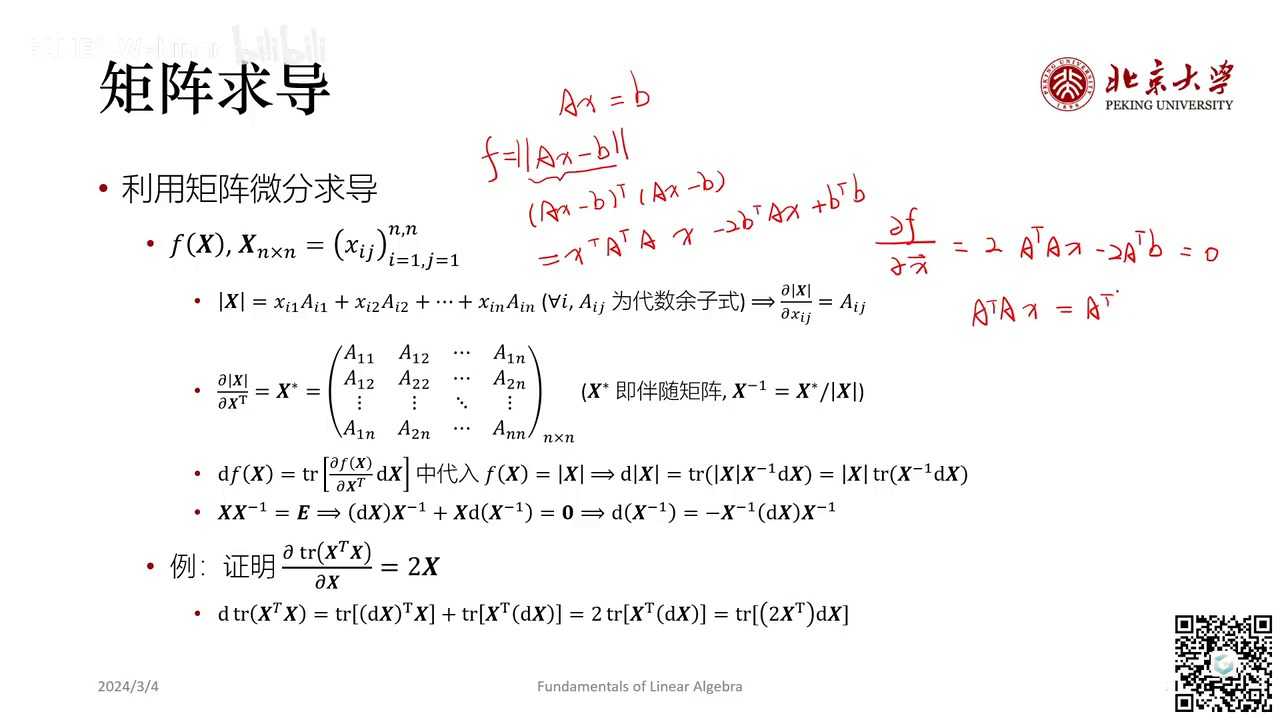
\includegraphics[width=0.92\textwidth]{figures/fig_17_least_squares.jpg}
\caption{手写板上的最小二乘推导：最小化 $\|\boldsymbol A\boldsymbol x-\boldsymbol b\|$ 得到 $\boldsymbol A^{\mathsf T}\boldsymbol A\boldsymbol x=\boldsymbol A^{\mathsf T}\boldsymbol b$\vtag}
\end{figure}
\srcnote{01:21:00--01:21:15}
\end{minipage}


\begin{knowledgebox}{去哪里查矩阵导数}
讲者推荐两类工具：一是 Kaare Petersen 与 Michael Pedersen 的《The Matrix Cookbook》，可以当工具书查各种矩阵导数；二是网站 matrixcalculus.org，可以直接输入表达式求导。他的看法是，这些结论多数并不繁琐，推一遍就会发现是“显见的”。
\end{knowledgebox}

\subsection{本章小结}

矩阵微分把求导转化为“整理微分式”：乘积法则展开、迹的轮换把 $\mathrm d\boldsymbol X$ 移到右边，左侧矩阵就是导数。行列式的导数给出伴随矩阵，逆矩阵的微分给出 $-\boldsymbol X^{-1}\mathrm d\boldsymbol X\boldsymbol X^{-1}$，最小二乘则自然导出正规方程与伪逆。下一章回到向量的乘法，说明点乘、叉乘与外积的区别。

\section{内积、叉积与外积}

\subsection{内积（标量积）}

内积又称标量积，两个向量相乘得到一个标量：
\[
\boldsymbol a\cdot\boldsymbol b=\langle\boldsymbol a,\boldsymbol b\rangle=\|\boldsymbol a\|\,\|\boldsymbol b\|\cos\theta ,
\]
\begin{itemize}
\item $\theta$：两向量的夹角；$\|\cdot\|$：向量模长。
\end{itemize}
其值为两向量模长之积乘以夹角余弦。

\subsection{叉积（向量积）}

叉积又称向量积，结果是一个向量：
\[
\|\boldsymbol a\times\boldsymbol b\|=\|\boldsymbol a\|\,\|\boldsymbol b\|\sin\theta,\qquad \boldsymbol a\cdot(\boldsymbol a\times\boldsymbol b)=0,\quad \boldsymbol b\cdot(\boldsymbol a\times\boldsymbol b)=0 .
\]
\begin{itemize}
\item $\boldsymbol a\times\boldsymbol b$：叉积，方向垂直于原来两个向量，正反由右手螺旋定则确定；大小为两向量模长之积乘以夹角正弦。
\end{itemize}
二维时（“伪”叉积）结果是实数 $(a_x,a_y)\times(b_x,b_y)=a_xb_y-b_xa_y$；三维时可以写成行列式
\[
(a_x,a_y,a_z)\times(b_x,b_y,b_z)=\begin{vmatrix}\boldsymbol e_x&\boldsymbol e_y&\boldsymbol e_z\\a_x&a_y&a_z\\b_x&b_y&b_z\end{vmatrix}.
\]
\begin{itemize}
\item $\boldsymbol e_x,\boldsymbol e_y,\boldsymbol e_z$：单位正交基；按第一行展开即得叉积的三个分量。
\end{itemize}

\noindent\begin{minipage}{\textwidth}
\begin{figure}[H]
\centering
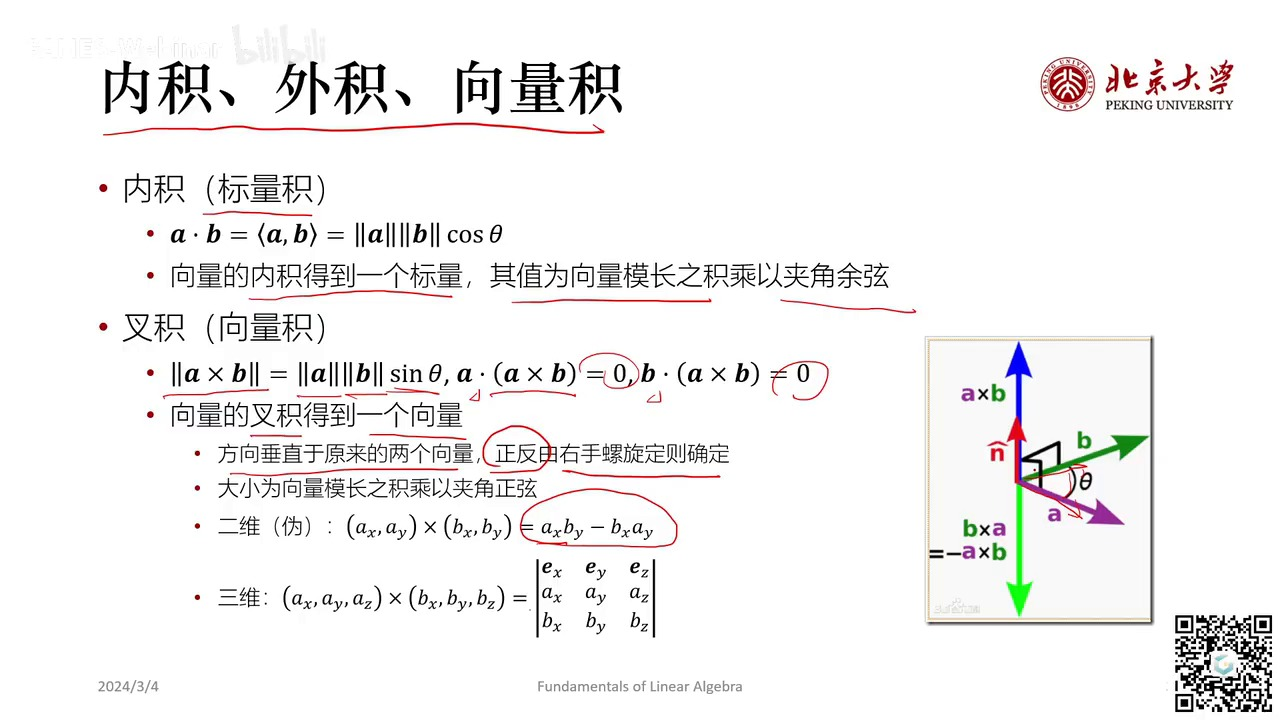
\includegraphics[width=0.92\textwidth]{figures/fig_18_dot_cross.jpg}
\caption{内积、叉积与右手螺旋定则：$\boldsymbol a\times\boldsymbol b$ 与 $\boldsymbol b\times\boldsymbol a=-\boldsymbol a\times\boldsymbol b$\vtag}
\end{figure}
\srcnote{01:25:30--01:25:45}
\end{minipage}


叉积还可以写成矩阵乘法。叉乘矩阵是一个反对称矩阵（$\boldsymbol A+\boldsymbol A^{\mathsf T}=\boldsymbol 0$）：
\[
\boldsymbol a\times\boldsymbol b=\boldsymbol A\boldsymbol b=\begin{pmatrix}0&-a_z&a_y\\a_z&0&-a_x\\-a_y&a_x&0\end{pmatrix}\begin{pmatrix}b_x\\b_y\\b_z\end{pmatrix}.
\]
\begin{itemize}
\item $\boldsymbol A$：由 $\boldsymbol a$ 构造的叉乘矩阵；$\boldsymbol b$：被叉乘的向量。
\end{itemize}

\subsection{外积（张量积）}

讲者纠正了一个常见的错误说法：外积并不是叉积。外积又称张量积，
\[
\boldsymbol a\otimes\boldsymbol b=\boldsymbol A=\boldsymbol a\boldsymbol b^{\mathrm H},\qquad
\begin{pmatrix}a_x\\a_y\\a_z\end{pmatrix}\begin{pmatrix}b_x&b_y&b_z\end{pmatrix}=\begin{pmatrix}a_xb_x&a_xb_y&a_xb_z\\a_yb_x&a_yb_y&a_yb_z\\a_zb_x&a_zb_y&a_zb_z\end{pmatrix},
\]
\begin{itemize}
\item $\boldsymbol a\otimes\boldsymbol b$：外积，列向量乘行向量，结果是矩阵；右式为实数域上的矩阵表示。
\end{itemize}
其性质为 $\operatorname{tr}(\boldsymbol a\otimes\boldsymbol b)=\boldsymbol a\cdot\boldsymbol b$。讲者把内积与外积对照起来：内积是行向量乘列向量（$\boldsymbol a^{\mathsf T}\boldsymbol b$），外积是列向量乘行向量（$\boldsymbol a\boldsymbol b^{\mathsf T}$），后者每个元素就是两向量对应分量的乘积。课件还在旁边列出了克罗内克（Kronecker）积：$\boldsymbol A_{m\times n}\otimes\boldsymbol B_{p\times q}$ 是把 $\boldsymbol A$ 的每个元素 $a_{ij}$ 换成分块 $a_{ij}\boldsymbol B$ 得到的大矩阵。

\noindent\begin{minipage}{\textwidth}
\begin{figure}[H]
\centering
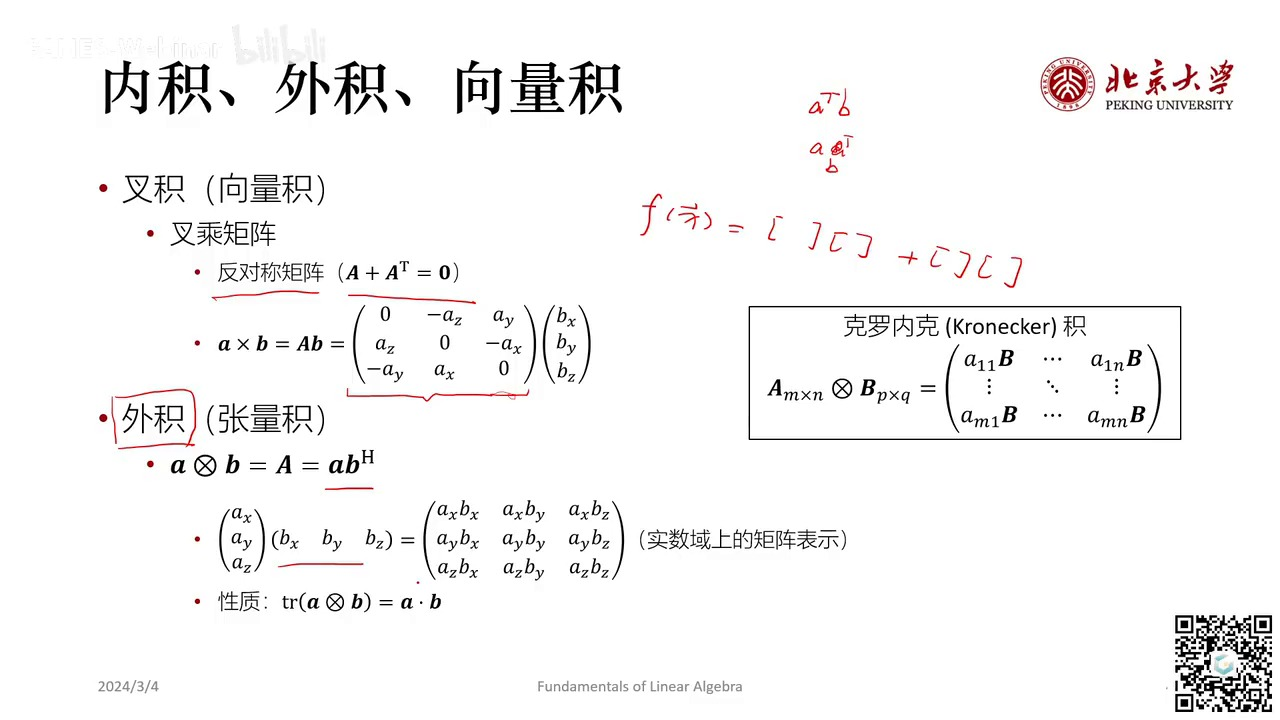
\includegraphics[width=0.92\textwidth]{figures/fig_19_cross_matrix_outer.jpg}
\caption{叉乘矩阵、外积（张量积）与克罗内克积\vtag}
\end{figure}
\srcnote{01:28:15--01:28:30}
\end{minipage}


\begin{center}
\begin{tabular}{p{0.18\textwidth}p{0.25\textwidth}p{0.18\textwidth}p{0.27\textwidth}}
\toprule
运算 & 记号 & 结果 & 要点 \\
\midrule
内积（标量积） & $\boldsymbol a\cdot\boldsymbol b=\boldsymbol a^{\mathsf T}\boldsymbol b$ & 标量 & $\|\boldsymbol a\|\|\boldsymbol b\|\cos\theta$ \\
叉积（向量积） & $\boldsymbol a\times\boldsymbol b$ & 向量（三维） & 垂直于两向量，模长 $\|\boldsymbol a\|\|\boldsymbol b\|\sin\theta$ \\
外积（张量积） & $\boldsymbol a\otimes\boldsymbol b=\boldsymbol a\boldsymbol b^{\mathrm H}$ & 矩阵 & 迹等于内积 \\
克罗内克积 & $\boldsymbol A\otimes\boldsymbol B$ & 分块大矩阵 & 每个元素替换为 $a_{ij}\boldsymbol B$ \\
\bottomrule
\end{tabular}
\end{center}

\subsection{本章小结}

三种“向量乘法”的结果分别是标量、向量与矩阵：内积给出夹角，叉积给出法向，外积把两个向量组合成一个二阶对象。外积已经预示了张量：当基底显式参与运算时，向量的乘法就变成张量的运算。

\section{张量：让基底显式参与运算}

讲者说，学线性代数时基底常常被我们忽略，但讲张量时会明显感受到基底很重要：它一直参与运算，帮助我们更清楚地理解线性空间与线性变换。

\subsection{协变与逆变}

在向量空间中，基底是人为给定的，本质的东西是向量本身；协变（covariant）与逆变（contravariant）是对分量而言的。以三维欧氏空间中的位移为例，$\boldsymbol x=x^1\boldsymbol e_1+x^2\boldsymbol e_2+x^3\boldsymbol e_3$，即沿 $\boldsymbol e_1$ 方向位移 $x^1$，沿 $\boldsymbol e_2$ 方向位移 $x^2$，沿 $\boldsymbol e_3$ 方向位移 $x^3$。
\begin{itemize}
\item 如果 $\boldsymbol e_i$ 的模长增大，坐标 $x^i$ 相应减小，因此称 $x^i$ 是“逆变”的；
\item 如果 $\boldsymbol e_i$ 的模长增大，$x_i=\boldsymbol x\cdot\boldsymbol e_i$ 也会增大，因此称 $x_i$ 是“协变”的。
\end{itemize}
一般情况下 $x_i\neq x^i$。可以定义一组新的基底 $(\boldsymbol e^1,\boldsymbol e^2,\boldsymbol e^3)$（注意下标变成了上标），使
\[
\boldsymbol e_i\cdot\boldsymbol e^j=\delta_i^j=\begin{cases}0,&i\neq j\\1,&i=j\end{cases},
\]
\begin{itemize}
\item $\delta_i^j$：克罗内克符号；$\boldsymbol e^j$：与原基底对偶的新基底。
\end{itemize}
于是位移也可以用逆变基底展开：$\boldsymbol x=x_1\boldsymbol e^1+x_2\boldsymbol e^2+x_3\boldsymbol e^3$。按爱因斯坦求和约定，上下重复的指标表示求和，记作 $\boldsymbol x=x_i\boldsymbol e^i=x^i\boldsymbol e_i$。

\begin{knowledgebox}{爱因斯坦求和约定}
同一项中一个指标在上、一个在下重复出现时，默认对该指标从 1 到维数求和，求和号省略不写。例如 $x^i\boldsymbol e_i$ 表示 $\sum_{i=1}^{3}x^i\boldsymbol e_i$。在单位正交基下上下标不再区分，重复下标即表示求和。
\end{knowledgebox}逆变与协变分量的关系为
\[
x_i=\boldsymbol x\cdot\boldsymbol e_i,\quad x^i=\boldsymbol x\cdot\boldsymbol e^i\ \Rightarrow\ x_i=(x^j\boldsymbol e_j)\cdot\boldsymbol e_i=x^j(\boldsymbol e_j\cdot\boldsymbol e_i)=x^jg_{ij},
\]
\begin{itemize}
\item $g_{ij}=\boldsymbol e_i\cdot\boldsymbol e_j$：度规张量，$i,j$ 各取 1、2、3，共九个分量。
\end{itemize}
讲者强调，常听到“逆变矢量”“协变矢量”的说法并不准确：矢量本身就是矢量，协变或逆变的只是它的分量。

\noindent\begin{minipage}{\textwidth}
\begin{figure}[H]
\centering
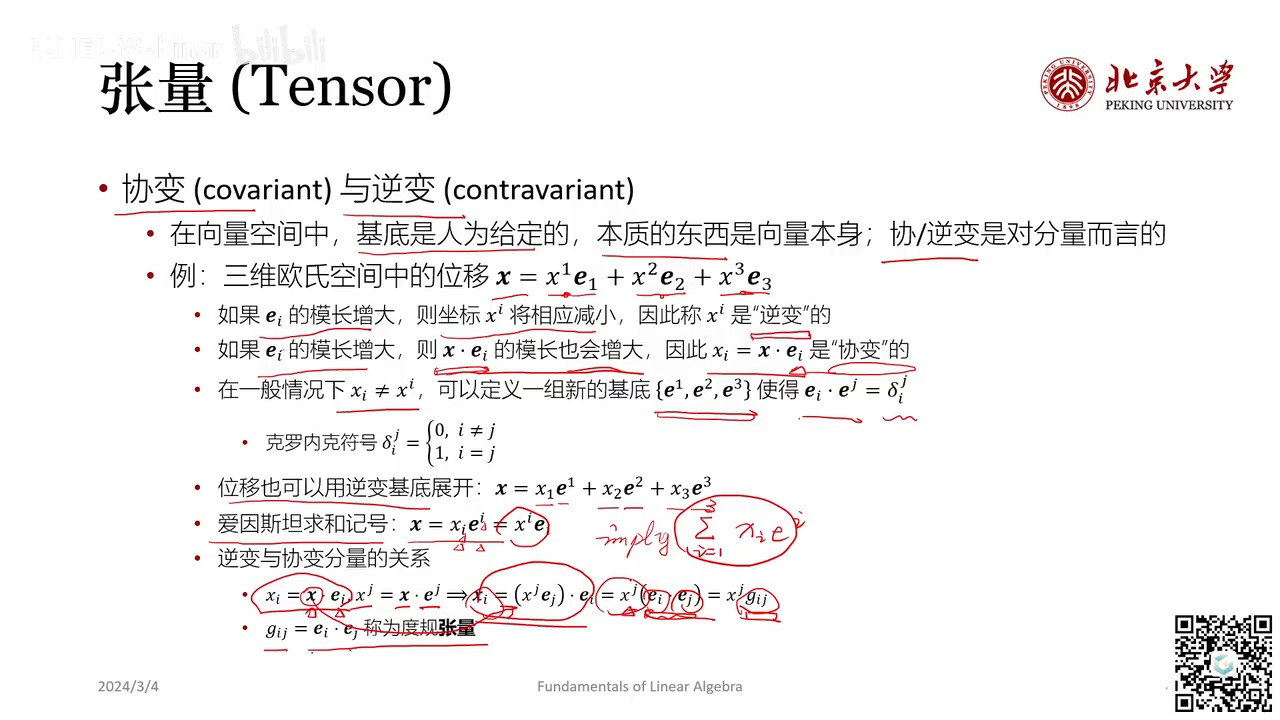
\includegraphics[width=0.92\textwidth]{figures/fig_20_covariant_contravariant.jpg}
\caption{协变与逆变：以位移为例，基底模长增大时逆变分量减小、协变分量增大，二者通过度规张量 $g_{ij}$ 联系\vtag}
\end{figure}
\srcnote{01:35:15--01:35:30}
\end{minipage}


\subsection{从标量、矢量到张量}

协变与逆变的概念由基底的选取而产生。标量（0 阶张量）没有“分量”的概念，因此无所谓协变或逆变；矢量（1 阶张量）是协变或逆变基底的线性组合，只有一个“指标”决定协变或逆变；张量（2 阶张量）有两个指标。例如克罗内克符号 $\delta_i^j$ 是 2 阶张量，1 阶逆变、1 阶协变，又称为 $(1,1)$ 阶混合张量。坐标变换下，各类张量的分量按如下规律变化：
\[
T^{\mu\nu}=\frac{\partial x^\mu}{\partial\bar x^\alpha}\frac{\partial x^\nu}{\partial\bar x^\beta}\bar T^{\alpha\beta},\qquad
T^{\mu}_{\nu}=\frac{\partial x^\mu}{\partial\bar x^\alpha}\frac{\partial\bar x^\beta}{\partial x^\nu}\bar T^{\alpha}_{\beta},
\]
\begin{itemize}
\item $T^{\mu\nu}$：$(2,0)$ 张量的分量；$T^{\mu}_{\nu}$：$(1,1)$ 张量的分量；带横线的量为另一坐标系下的分量；偏导数为两坐标系之间的变换系数。
\end{itemize}
课件提出一个问题：矩阵是如何表示线性变换的？答案是：基底不变、更改坐标时，矩阵元构成 $(2,0)$ 阶张量；坐标不变、更改基底时，矩阵元构成 $(0,2)$ 阶张量。讲者补充：不管用 $(2,0)$ 阶还是 $(0,2)$ 阶，都能表示所有的线性变换，只是理解线性变换的方式不同。

\noindent\begin{minipage}{\textwidth}
\begin{figure}[H]
\centering
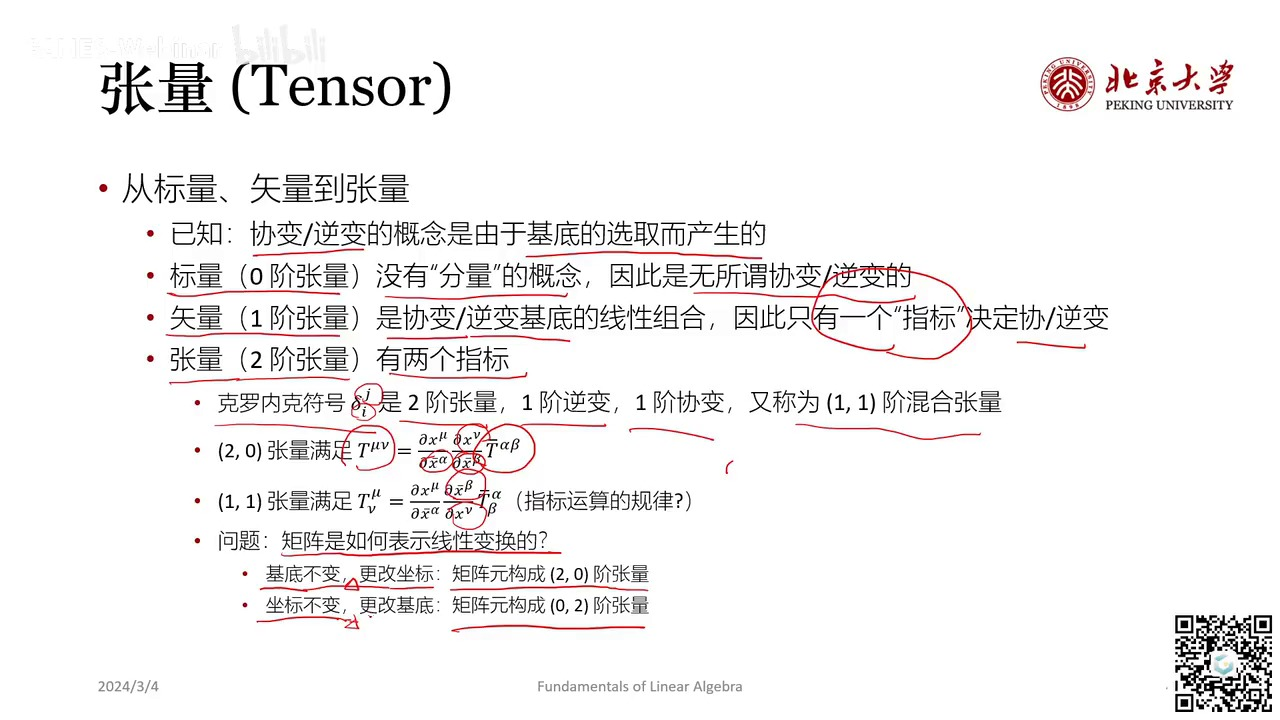
\includegraphics[width=0.92\textwidth]{figures/fig_21_tensor_order.jpg}
\caption{从标量、矢量到张量：协变/逆变的指标，$(2,0)$ 与 $(1,1)$ 张量的变换规律，以及矩阵作为张量的两种理解\vtag}
\end{figure}
\srcnote{01:39:15--01:39:30}
\end{minipage}


\subsection{并矢与张量的并乘}

并矢（dyadic tensor）是物理上对两向量张量积的直观理解。例如 $\boldsymbol x=a\boldsymbol i+b\boldsymbol j$，$\boldsymbol y=c\boldsymbol i+d\boldsymbol j$，其并矢为
\[
\boldsymbol x\boldsymbol y=ac\,\boldsymbol i\boldsymbol i+ad\,\boldsymbol i\boldsymbol j+bc\,\boldsymbol j\boldsymbol i+bd\,\boldsymbol j\boldsymbol j,\qquad
\boldsymbol x\boldsymbol y\cdot\boldsymbol z=\boldsymbol x(\boldsymbol y\cdot\boldsymbol z),\quad \boldsymbol x\cdot\boldsymbol y\boldsymbol z=(\boldsymbol x\cdot\boldsymbol y)\boldsymbol z ,
\]
\begin{itemize}
\item $\boldsymbol i,\boldsymbol j$：基底；$\boldsymbol i\boldsymbol j$ 等：基底的并矢；后两式为并矢与点积的结合律，可以用张量积的矩阵形式证明。
\end{itemize}
并矢的分量形式是 $t^{ij}=x^iy^j$，是一个 $(2,0)$ 阶张量，对应矩阵 $\boldsymbol x\boldsymbol y^{\mathsf T}$。讲者说明，并矢并不是非常严格定义的概念，它与张量分析之间有一定差别。

从张量分析的角度，可以定义张量的并乘：$(m,n)$ 阶张量与 $(p,q)$ 阶张量并乘得到 $(m+p,n+q)$ 阶张量。例如 $\boldsymbol x=x^i\boldsymbol e_i$，$\boldsymbol y=y^j\boldsymbol e_j$，并乘得到 $t^{ij}=x^iy^j$，$\boldsymbol T=\boldsymbol x\boldsymbol y=x^i\boldsymbol e_iy^j\boldsymbol e_j=x^iy^j\boldsymbol e_i\boldsymbol e_j$。做法是把分量提出来写在一起，把基底按顺序写在后面；讲者强调，基底的顺序不能交换。

\noindent\begin{minipage}{\textwidth}
\begin{figure}[H]
\centering
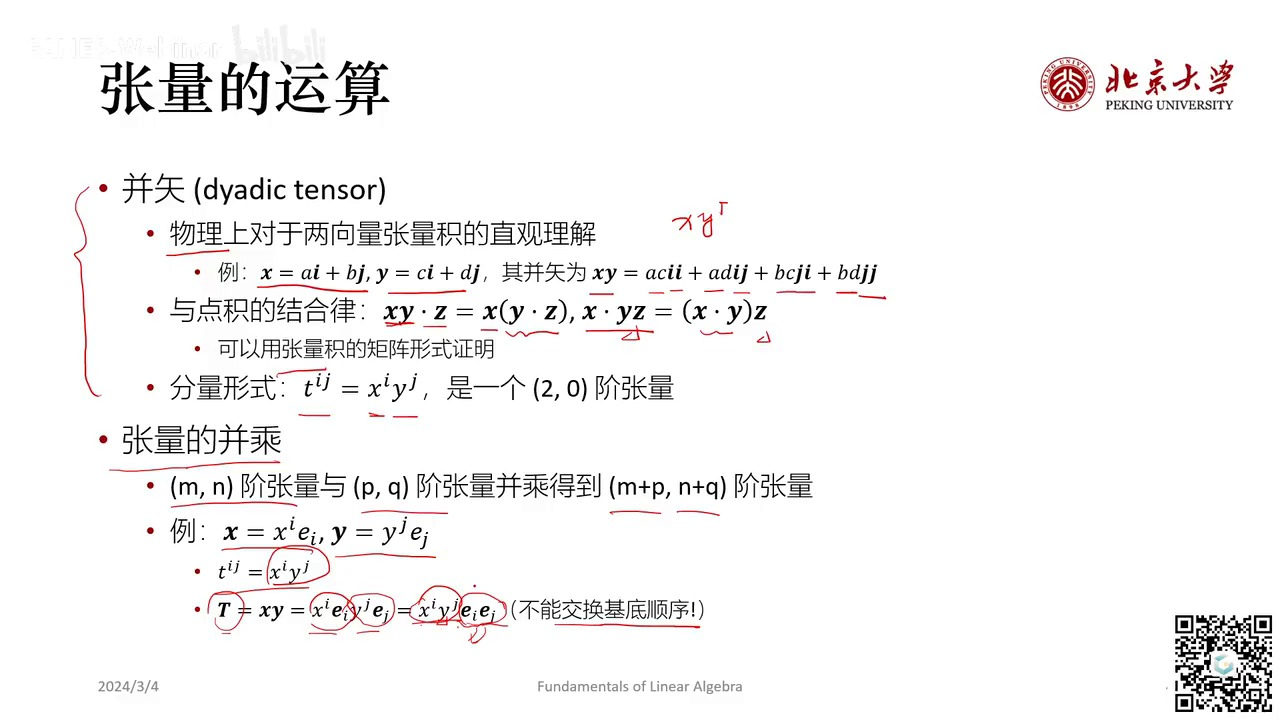
\includegraphics[width=0.92\textwidth]{figures/fig_22_dyadic_product.jpg}
\caption{张量的运算：并矢及其与点积的结合律，以及张量的并乘\vtag}
\end{figure}
\srcnote{01:42:15--01:42:30}
\end{minipage}


\subsection{缩并与点积}

缩并是张量运算中降阶的操作。例如 $\boldsymbol T=x^iy^jz_k\boldsymbol e_i\boldsymbol e_j\boldsymbol e^k$，缩并 $\boldsymbol e_j$ 与 $\boldsymbol e^k$：
\[
x^iy^jz_k\boldsymbol e_i\delta_j^k=x^iy^jz_j\boldsymbol e_i ,
\]
\begin{itemize}
\item $\delta_j^k$：把一对协变/逆变基底的点积替换成克罗内克符号；求和后指标 $k$ 被 $j$ 取代。
\end{itemize}
缩并一般在一对协变与逆变基底之间展开，利用克罗内克符号使张量阶数降低 2。缩并后的张量与被缩并的基底无关：无论 $\boldsymbol e_i$ 与 $\boldsymbol e_j$ 如何选取，都不再影响缩并后张量的形式。课件举例：三维空间中 $a_i^j\boldsymbol e^i\boldsymbol e_j$ 的缩并结果为 0 阶张量 $a_1^1+a_2^2+a_3^3$，这是一个与基底选取无关的量，也就是迹。讲者把它和上一讲连起来：迹不随相似变换而改变，正是因为它是缩并的结果。

两个张量 $\boldsymbol T,\boldsymbol S$ 的点积等于它们先并联、再缩并的结果。点积的形式有多种；当选择缩并 $\boldsymbol T$ 的最后一个基矢与 $\boldsymbol S$ 的第一个基矢时，记为 $\boldsymbol T\cdot\boldsymbol S$。双点积则缩并两对基矢，分两种：并联式先缩并 $\boldsymbol T$ 与 $\boldsymbol S$ 的倒数第一个基矢、再缩并倒数第二个基矢；串联式先缩并 $\boldsymbol T$ 的倒数第一个与 $\boldsymbol S$ 的第一个基矢、再缩并 $\boldsymbol T$ 与 $\boldsymbol S$ 中间的基矢（讲者在课上一度把两者说反，随即更正）：
\[
\boldsymbol T:\boldsymbol S=(t^{ij}\boldsymbol e_i\boldsymbol e_j):(s_{kl}\boldsymbol e^k\boldsymbol e^l)=t^{ij}s_{kl}\delta_i^k\delta_j^l,\qquad
\boldsymbol T\cdot\cdot\,\boldsymbol S=(t^{ij}\boldsymbol e_i\boldsymbol e_j)\cdot\cdot\,(s_{kl}\boldsymbol e^k\boldsymbol e^l)=t^{ij}s_{kl}\delta_j^k\delta_i^l .
\]
\begin{itemize}
\item $\boldsymbol T:\boldsymbol S$：并联式双点积；$\boldsymbol T\cdot\cdot\,\boldsymbol S$：串联式双点积；$t^{ij},s_{kl}$：两张量的分量。
\end{itemize}

\noindent\begin{minipage}{\textwidth}
\begin{figure}[H]
\centering
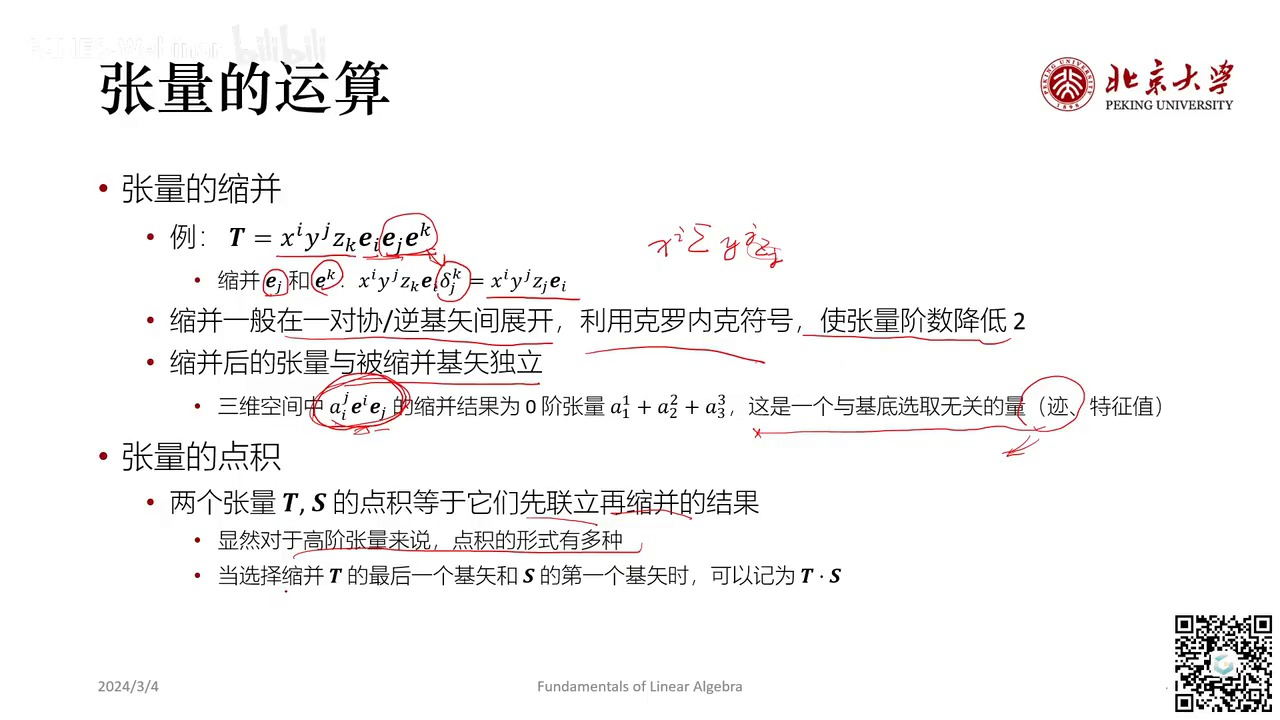
\includegraphics[width=0.92\textwidth]{figures/fig_23_contraction.jpg}
\caption{张量的缩并与点积：缩并降低两阶且与基底选取无关，三维中 $a_i^j\boldsymbol e^i\boldsymbol e_j$ 的缩并即迹\vtag}
\end{figure}
\srcnote{01:45:30--01:45:45}
\end{minipage}


\subsection{实例：结合律与物质导数中的对流项}

课件给出两个实例。第一个是并矢与点积的结合律：
\[
\boldsymbol x\boldsymbol y\cdot\boldsymbol z=(x^iy^j\boldsymbol e_i\boldsymbol e_j)\cdot(z_k\boldsymbol e^k)=x^iy^jz_k\boldsymbol e_i\delta_j^k=x^iy^jz_j\boldsymbol e_i=\boldsymbol x(\boldsymbol y\cdot\boldsymbol z).
\]
\begin{itemize}
\item 先把每个向量写成分量乘基底，按顺序并联，再缩并相邻的一对基底。
\end{itemize}
第二个与流体模拟有关：
\[
\boldsymbol u\cdot\nabla\boldsymbol u=(u_i\boldsymbol e^i)\cdot\left(\left(\boldsymbol e_j\frac{\partial}{\partial x^j}\right)(u^k\boldsymbol e_k)\right)=u_i\delta_j^i\frac{\partial u^k}{\partial x^j}\boldsymbol e_k=\left(u_j\frac{\partial}{\partial x^j}\right)(u^k\boldsymbol e_k)=(\boldsymbol u\cdot\nabla)\boldsymbol u ,
\]
\begin{itemize}
\item $\boldsymbol u$：速度场；$\nabla=\boldsymbol e_j\,\partial/\partial x^j$：梯度算子；$\partial/\partial x^j$ 可简记为 $\partial_j$，$\partial u^k/\partial x^j$ 可简记为 $u^k_{,j}$。
\end{itemize}
当 $\boldsymbol u$ 为速度场时，这一项是物质导数（随体导数）的重要部分。讲者解释，它出现在纳维—斯托克斯方程左侧：流体中的量不仅自身在变，还在沿着速度场移动，所以要多加一项描述“沿速度场的运动”。

\noindent\begin{minipage}{\textwidth}
\begin{figure}[H]
\centering
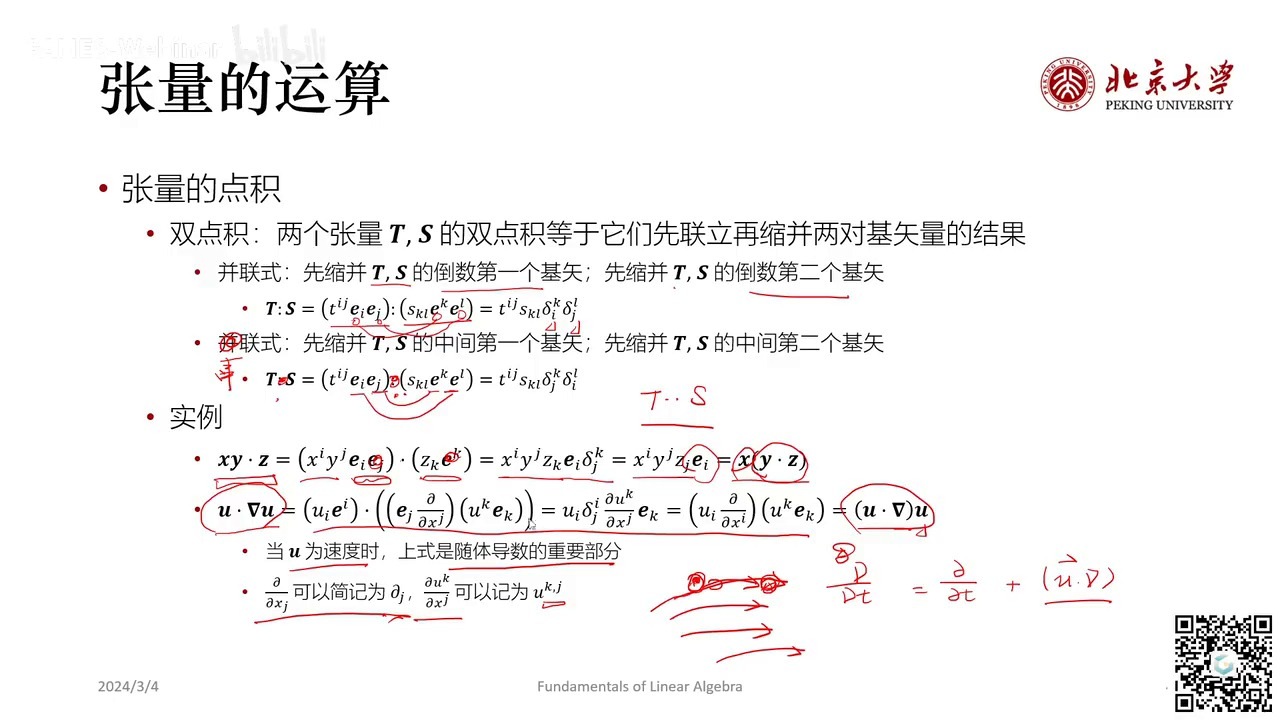
\includegraphics[width=0.92\textwidth]{figures/fig_24_tensor_examples.jpg}
\caption{张量点积的实例：并矢结合律的证明，以及流体模拟中 $\boldsymbol u\cdot\nabla\boldsymbol u=(\boldsymbol u\cdot\nabla)\boldsymbol u$\vtag}
\end{figure}
\srcnote{01:50:45--01:51:00}
\end{minipage}


\subsection{Levi-Civita 符号与叉积}

为了用张量表示叉积，需要引入列维—奇维塔（Levi-Civita）符号 $\epsilon_{ijk}$。它是一个三阶张量：
\[
\epsilon_{ijk}=\epsilon_{jki}=\epsilon_{kij}=1,\qquad \epsilon_{kji}=\epsilon_{ikj}=\epsilon_{jik}=-1,\qquad \text{下标有重复时为 }0 ,
\]
\begin{itemize}
\item 在 $(i,j,k)=(1,2,3)$ 的偶置换上取 $1$，奇置换上取 $-1$。
\end{itemize}
其性质为
\[
\epsilon_{ijk}\epsilon^{lmn}=\delta_i^l\delta_j^m\delta_k^n-\cdots,\qquad
\epsilon_{ijk}\epsilon^{imn}=\delta_j^m\delta_k^n-\delta_j^n\delta_k^m,\qquad
\epsilon_{ijk}\epsilon^{ijn}=2\delta_k^n,\qquad
\epsilon_{ijk}\epsilon^{ijk}=6 ,
\]
\begin{itemize}
\item 第一式右侧是以克罗内克符号为元素的 $3\times3$ 行列式展开（课件只写出首项）；后三式依次缩并一对、两对、三对指标。
\end{itemize}
讲者说明了最后一式：当 $i,j,k$ 分别从 1 取到 3 时，只有六种排列使 $\epsilon_{ijk}$ 非零，每种的平方都是 1，所以结果是 6。一般意义下，该符号表达的是各指标的排列的奇偶性，因此也可以用来定义行列式。

用 Levi-Civita 符号，叉积写成
\[
\boldsymbol x\times\boldsymbol y=(x^i\boldsymbol e_i)\times(y^j\boldsymbol e_j)=x^iy^j\epsilon_{ij}^{\ \ k}\boldsymbol e_k ,
\]
\begin{itemize}
\item $\epsilon_{ij}^{\ \ k}$：Levi-Civita 符号；在单位正交基底下可以忽略协变与逆变，记为 $(\boldsymbol x\times\boldsymbol y)_k=x_iy_j\epsilon_{ijk}$。
\end{itemize}
作为示例，课件证明了拉格朗日恒等式：
\[
\|\boldsymbol x\times\boldsymbol y\|^2=x^iy^jx_my_n\epsilon_{ijk}\epsilon^{mnk}=x^iy^jx_my_n(\delta_i^m\delta_j^n-\delta_i^n\delta_j^m)=x^iy^jx_iy_j-x^iy^jx_jy_i=\|\boldsymbol x\|^2\|\boldsymbol y\|^2-(\boldsymbol x\cdot\boldsymbol y)^2 .
\]
\begin{itemize}
\item 第二步用了缩并一对指标的性质；第三步按克罗内克符号代换指标；最后识别出模长平方与内积平方。
\end{itemize}

\noindent\begin{minipage}{\textwidth}
\begin{figure}[H]
\centering
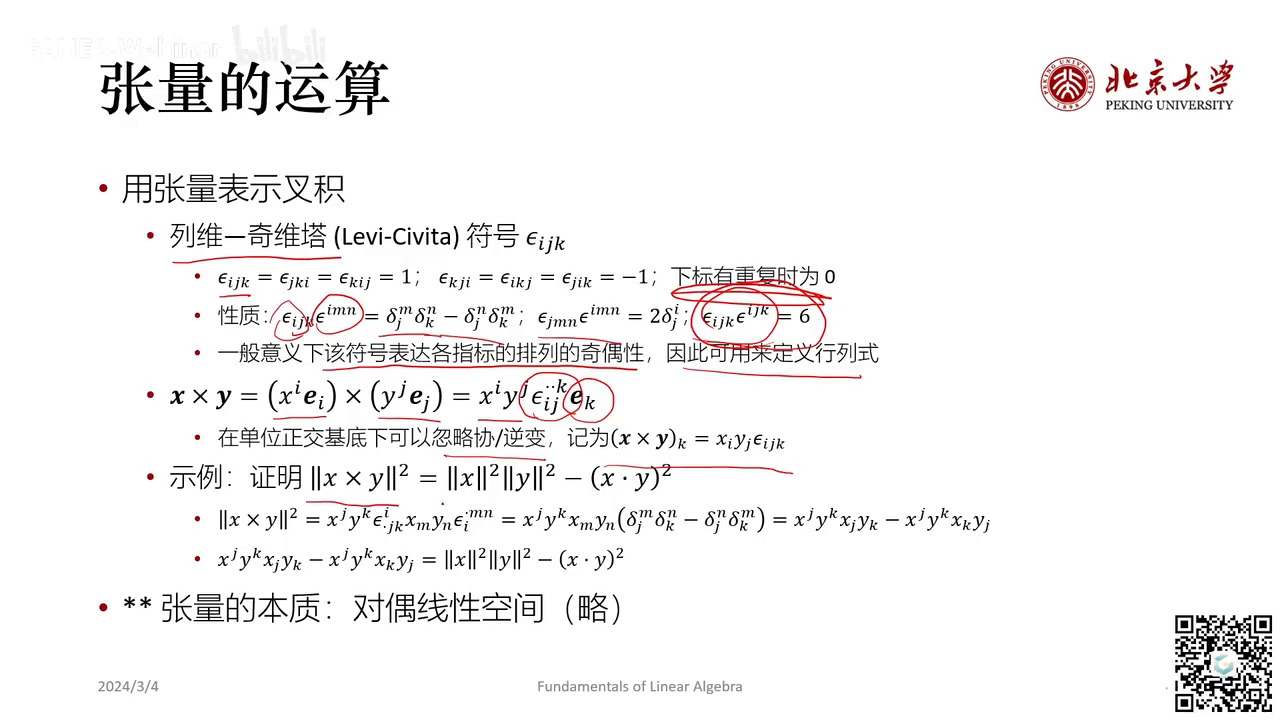
\includegraphics[width=0.92\textwidth]{figures/fig_25_levi_civita.jpg}
\caption{用张量表示叉积：Levi-Civita 符号的定义与性质，以及 $\|\boldsymbol x\times\boldsymbol y\|^2=\|\boldsymbol x\|^2\|\boldsymbol y\|^2-(\boldsymbol x\cdot\boldsymbol y)^2$ 的证明\vtag}
\end{figure}
\srcnote{01:53:30--01:53:45}
\end{minipage}


\noindent\begin{minipage}{\textwidth}
\begin{figure}[H]
\centering
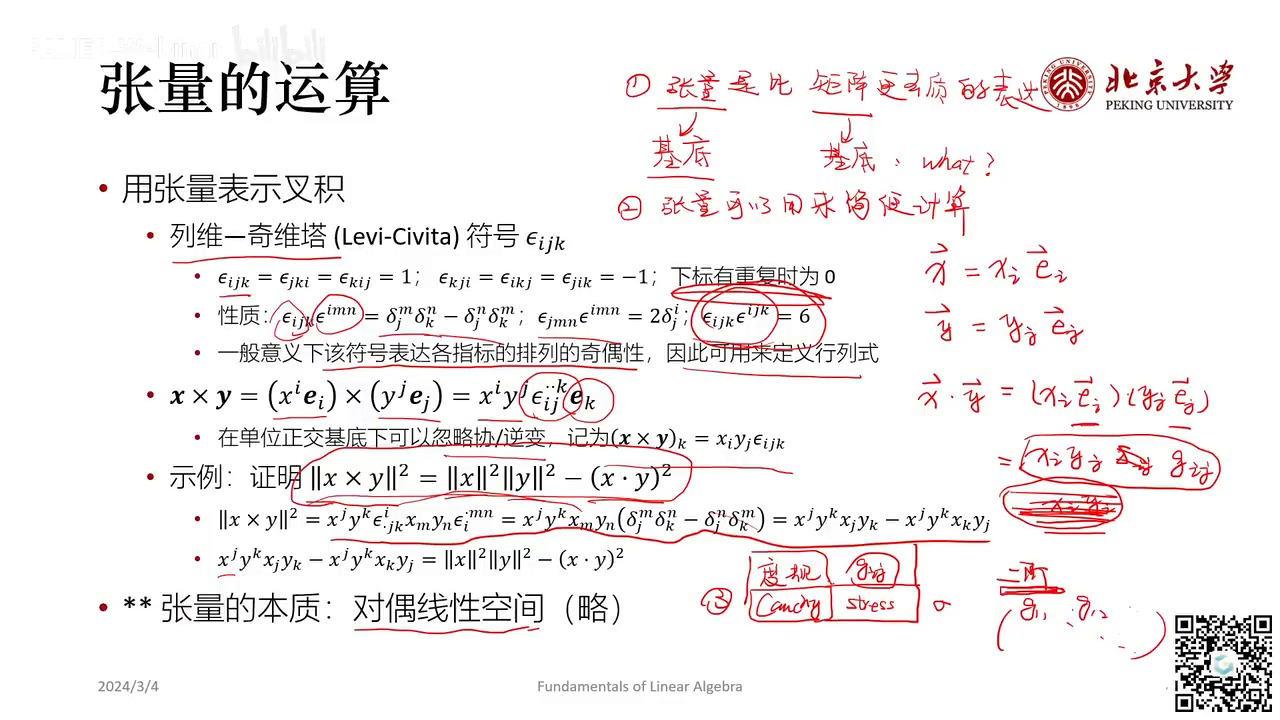
\includegraphics[width=0.92\textwidth]{figures/fig_26_levi_civita_annotated.jpg}
\caption{讲者在课件上手写标注 Levi-Civita 符号的取值与缩并过程\vtag}
\end{figure}
\srcnote{01:59:45--02:00:00}
\end{minipage}


\subsection{张量记号的意义}

讲者没有展开张量的本质（对偶线性空间），只分享了他的个人理解。在线性代数里，即使不知道基底是什么，也能做很多计算；但讲张量时，必须时刻记得对应的是协变分量、逆变分量，还是两者兼有。如果暂时不理解协变与逆变，至少可以这样用：写 $\boldsymbol x=x^i\boldsymbol e_i$、$\boldsymbol y=y^j\boldsymbol e_j$，计算 $\boldsymbol x\cdot\boldsymbol y$ 时把基底的点积换成度规张量 $g_{ij}$，在单位正交基下 $g_{ij}=\delta_{ij}$，最终得到 $x_iy_i$，这正是欧几里得空间中最熟悉的内积算法。

他总结了张量记号的两点价值：其一，统一了各种乘法与运算；其二，可以用来简便地证明恒等式，比如前面的拉格朗日恒等式，看到相同的下标就相乘求和。图形学里所谓的张量一般都是二阶的，二阶张量与矩阵表达的是同样的物理背景；他的建议是，觉得某个张量难以理解时，就尝试把它当成二阶张量（矩阵）去理解。

\begin{importantbox}{用张量记号做证明的步骤}
把每个向量写成“分量 $\times$ 基底”，按顺序并联；遇到点积就缩并一对基底并换成 $\delta$；遇到叉积就引入 $\epsilon_{ijk}$；利用 $\epsilon\epsilon$ 的缩并公式化简；最后把剩下的求和式识别为模长、内积或迹等不依赖基底的量。
\end{importantbox}

\subsection{本章小结}

张量把基底显式写进运算：分量分协变与逆变，度规张量连接两者；并乘升阶，缩并降阶，迹就是缩并；Levi-Civita 符号把叉积与行列式纳入同一套记号。掌握这些规则后，向量恒等式的证明变成机械的指标运算。

\section{总结与延伸}

\subsection{讲者的收尾与学习建议}

倪星宇在结尾推荐了拓展阅读：教科书有 Sheldon Axler 的《Linear Algebra Done Right》（2015）、Petersen 与 Pedersen 的《The Matrix Cookbook》（2012）、张贤达的《矩阵分析与应用》（第 2 版，2013）、黄克智等的《张量分析》（第 3 版，2020）以及弗兰克尔的《物理几何学导论》（2016）；网站有 3Blue1Brown 与 matrixcalculus.org。他特别推荐 3Blue1Brown 的线性代数视频，以非常直观的动画讲述线性代数；《The Matrix Cookbook》则可以作为工具书去查矩阵求导的结论。

作业为 7 道在图形学中有所应用的线性代数证明或计算题，用 LaTeX 或 Word 等工具规范排版，导出 PDF；满分 100 分，达到 60 分为通过，全部课程作业中通过 80\% 者可获得结业认证；通过在线课程系统提交，需在 2024 年 4 月 16 日 00:00 前提交，每次作业时限为五周。讲者说，线性代数如果不从理论角度讲，很多东西讲不清楚，所以前两讲只能作为“工具书”式的梳理；从下一讲（计算几何）开始，内容将进入与图形学关系更密切的数学专题。

\noindent\begin{minipage}{\textwidth}
\begin{figure}[H]
\centering
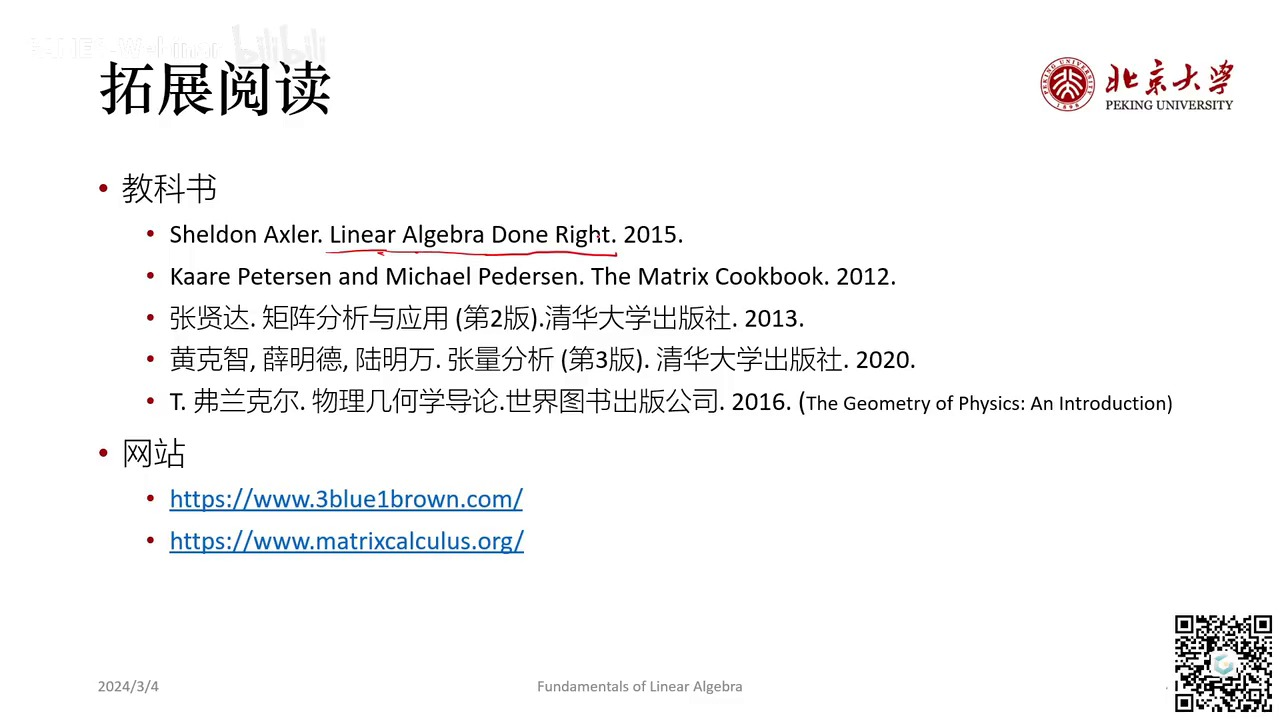
\includegraphics[width=0.92\textwidth]{figures/fig_27_further_reading.jpg}
\caption{拓展阅读：线性代数、矩阵分析与张量分析的教科书，以及 3Blue1Brown 与 matrixcalculus.org\vtag}
\end{figure}
\srcnote{02:02:00--02:02:15}
\end{minipage}


\noindent\begin{minipage}{\textwidth}
\begin{figure}[H]
\centering
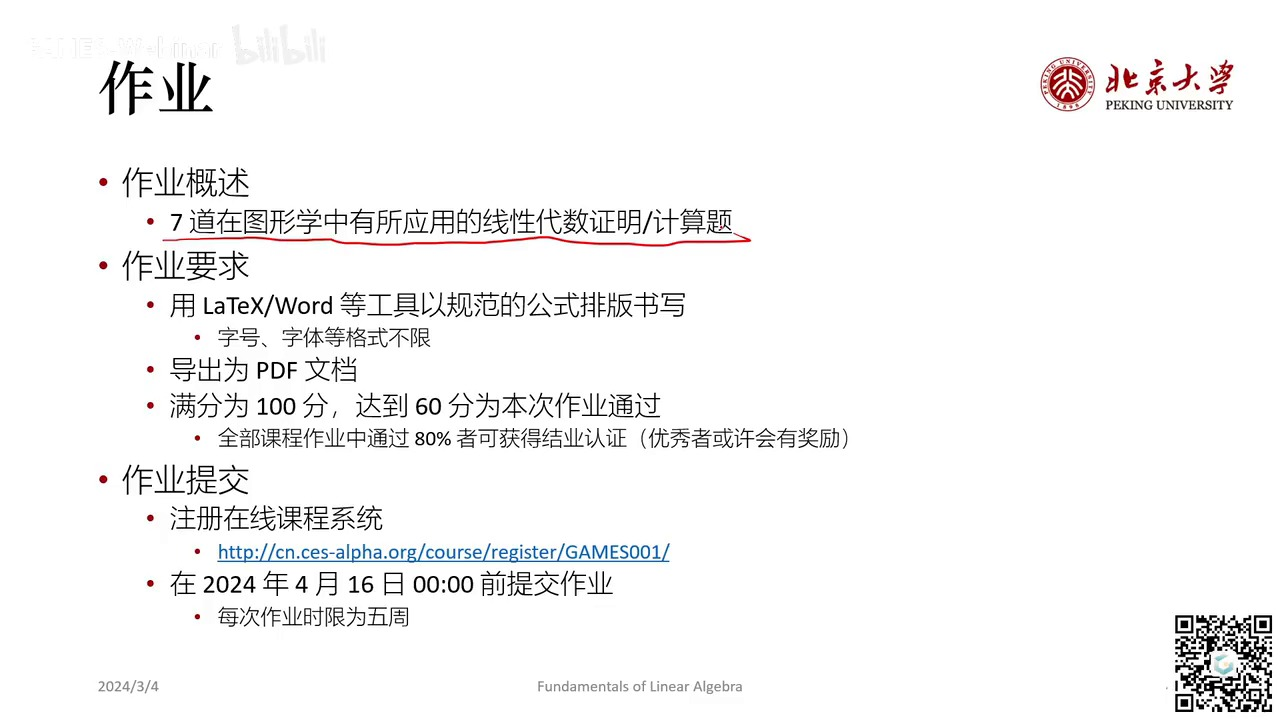
\includegraphics[width=0.92\textwidth]{figures/fig_28_homework.jpg}
\caption{第一次作业：7 道线性代数证明/计算题，2024 年 4 月 16 日前通过在线课程系统提交\vtag}
\end{figure}
\srcnote{02:04:00--02:04:15}
\end{minipage}


课后答疑中，讲者再次用一张课件梳理了求导的“形状”规则：标量对向量求偏导得到向量，对矩阵求偏导得到矩阵，每个元素是标量对相应分量的偏导；微分 $\mathrm df$ 的形状由因变量决定，与 $f$ 完全相同。

\noindent\begin{minipage}{\textwidth}
\begin{figure}[H]
\centering
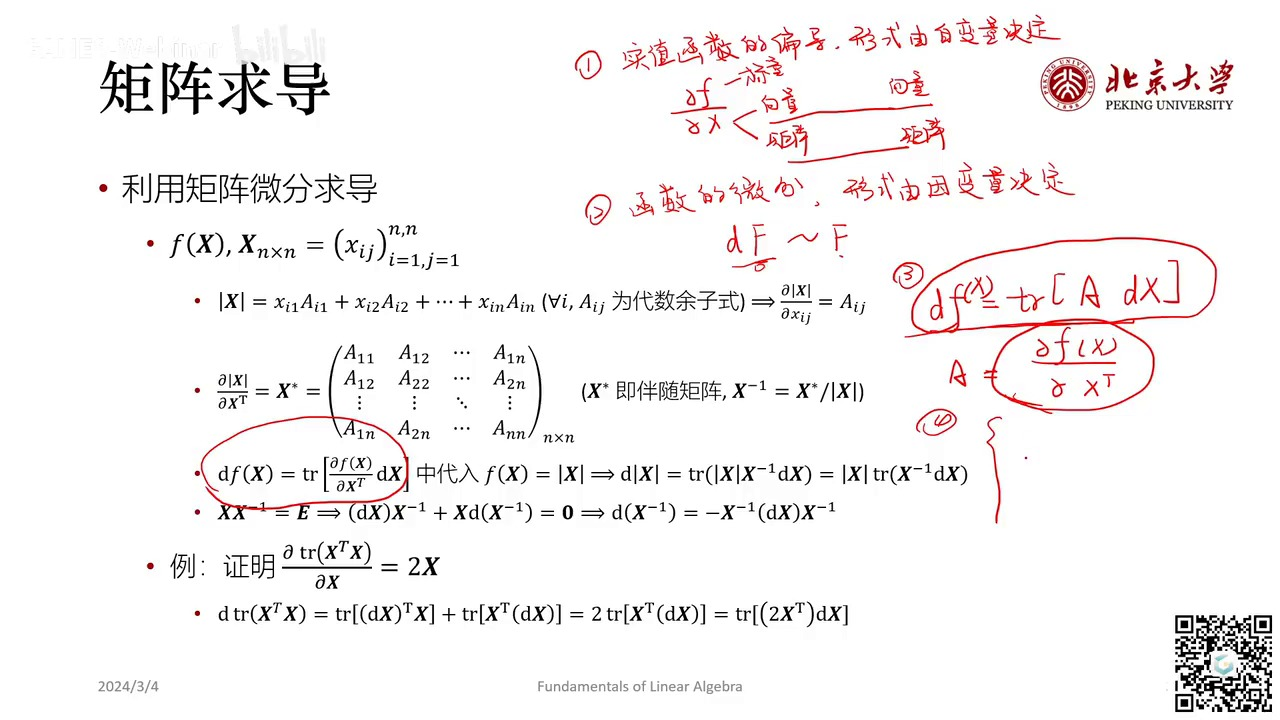
\includegraphics[width=0.92\textwidth]{figures/fig_29_qa_shape_rule.jpg}
\caption{答疑时的手写总结：偏导数的形状由自变量决定，微分的形状由因变量决定\vtag}
\end{figure}
\srcnote{02:13:00--02:13:15}
\end{minipage}


\subsection{讲义作者的归纳}

以下为讲义整理，不是讲者原话。第二讲的四个主题可以沿“求解—度量—求导—记号”串起来：
\begin{itemize}
\item \textbf{求解}：矩阵分解把方程变成三角回代或正交投影；Cholesky 依赖对称正定，QR 在物理模拟中剥离旋转，SVD 揭示任意变换都是“旋转—缩放—旋转”。
\item \textbf{度量}：向量范数是长度，矩阵的诱导范数是最大放大倍数，谱范数是最大奇异值；奇异值把 SVD 与范数连在一起。
\item \textbf{求导}：微分—迹法则是最实用的工具，它直接导出行列式、逆矩阵的导数和最小二乘的正规方程。
\item \textbf{记号}：张量把基底写进公式，迹是缩并、叉积是 Levi-Civita 符号的缩并，恒等式的证明因此变得机械。
\end{itemize}

\subsection{留给读者的问题}

\begin{itemize}
\item 证明 $\|\boldsymbol A\|_2=\sigma_{\max}(\boldsymbol A)$（课件留作作业）。
\item 用微分—迹法则推导 $\partial|\boldsymbol X|/\partial\boldsymbol X$ 与 $\partial\operatorname{tr}(\boldsymbol X^{-1}\boldsymbol A)/\partial\boldsymbol X$。
\item 当 $\boldsymbol A^{\mathsf T}\boldsymbol A$ 不可逆时，最小二乘解还唯一吗？SVD 如何给出此时的伪逆？
\item 用 Levi-Civita 符号证明 $\boldsymbol a\times(\boldsymbol b\times\boldsymbol c)=\boldsymbol b(\boldsymbol a\cdot\boldsymbol c)-\boldsymbol c(\boldsymbol a\cdot\boldsymbol b)$。
\end{itemize}

\end{document}
